\documentclass[aspectratio=169]{beamer}
\usetheme{Madrid}
\usecolortheme{seahorse}
\usepackage{amsmath}
\usepackage{amssymb}
\usepackage{graphicx}
\usepackage{tikz}
\usepackage{algorithm}
\usepackage{algorithmic}
\usepackage{xcolor}
\usepackage{soul}
\usetikzlibrary{shapes.geometric, arrows, positioning, calc}
\usepackage{newunicodechar}   % Allows you to define Unicode characters
\usepackage{pifont}
\newunicodechar{✓}{\checkmark}
\newunicodechar{✗}{\ding{55}}
\definecolor{warningcolor}{RGB}{255,0,0}
\definecolor{intuitioncolor}{RGB}{0,100,0}
\definecolor{ethicscolor}{RGB}{128,0,128}

\newcommand{\warning}[1]{\colorbox{red!10}{\textcolor{warningcolor}{\textbf{Warning:} #1}}}
\newcommand{\intuition}[1]{\colorbox{green!10}{\textcolor{intuitioncolor}{\textbf{Intuition:} #1}}}
\newcommand{\ethics}[1]{\colorbox{purple!10}{\textcolor{ethicscolor}{\textbf{Ethics:} #1}}}

\title{t-Stochastic Neighbor Embedding: A Journey from Information Theory to Responsible Visualization}
\author{Prof. Endri Raco}
\institute{Polytechnic University of Catalonia\\Guest Lecture - Advanced Multivariate Analysis}
\date{November 2025}

\begin{document}

% Slide 1
\begin{frame}
\titlepage
\end{frame}

\begin{frame}{Opening: The Fundamental Challenge We Face}
\begin{columns}
\column{0.5\textwidth}
\begin{center}
\textbf{High-D Space (10D)}\\
\vspace{0.3cm}
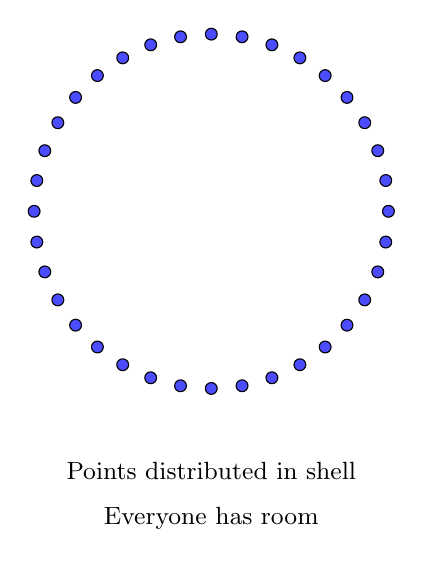
\begin{tikzpicture}[scale=1.5]
% Draw points in a shell pattern
\foreach \i in {0,10,...,350} {
    \draw[fill=blue!70] (\i:1.5cm) circle (0.05cm);
}
% Add label
\node at (0,-2.2) {\small Points distributed in shell};
\node at (0,-2.6) {\small Everyone has room};
\end{tikzpicture}
\end{center}

\column{0.5\textwidth}
\begin{center}
\textbf{Projected to 2D}\\
\vspace{0.3cm}
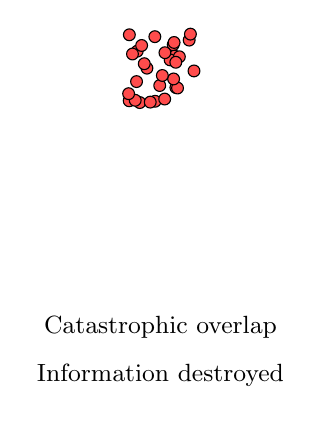
\begin{tikzpicture}[scale=1.5]
% Draw crowded points in center
\foreach \i in {1,...,30} {
    \pgfmathsetmacro\rx{rand*0.3}
    \pgfmathsetmacro\ry{rand*0.3}
    \draw[fill=red!70] (\rx,\ry) circle (0.05cm);
}
% Add label
\node at (0,-2.2) {\small Catastrophic overlap};
\node at (0,-2.6) {\small Information destroyed};
\end{tikzpicture}
\end{center}
\end{columns}

\vspace{0.5cm}
\begin{block}{The Paradox}
Your data lives in 784 dimensions. Your screen has 2.\\
\textbf{How do we preserve the essence when we must destroy the structure?}
\end{block}

\vspace{0.2cm}
\colorbox{yellow!20}{\parbox{0.95\textwidth}{\textbf{Key Insight:} Every visualization is a lie - our job is to make it the most honest lie possible}}
\end{frame}

\begin{frame}{Interactive Demonstration: The Crowding Catastrophe}
\begin{columns}
\column{0.45\textwidth}
\begin{center}
\textbf{High-D Space (10D)}\\
\vspace{0.2cm}
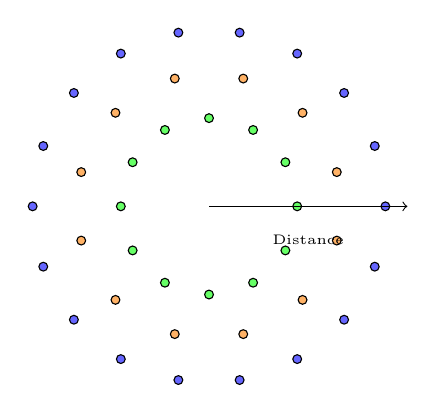
\begin{tikzpicture}[scale=1.4]
% Draw three concentric shells representing different distances
% Inner shell - near neighbors
\foreach \i in {0,30,...,330} {
    \draw[fill=green!60] (\i:0.8cm) circle (0.04cm);
}
% Middle shell - medium distance
\foreach \i in {15,45,...,345} {
    \draw[fill=orange!60] (\i:1.2cm) circle (0.04cm);
}
% Outer shell - far neighbors  
\foreach \i in {0,20,...,340} {
    \draw[fill=blue!60] (\i:1.6cm) circle (0.04cm);
}
\draw[->] (0,0) -- (1.8,0);
\node at (0.9,-0.3) {\tiny Distance};
\end{tikzpicture}
\vspace{0.2cm}

\textbf{Three distinct distance shells}\\
{\small Near \textcolor{green!60}{$ \bullet $} Medium \textcolor{orange!60}{$ \bullet $} Far \textcolor{blue!60}{$ \bullet $}}
\end{center}

\column{0.45\textwidth}
\begin{center}
\textbf{Projected to 2D}\\
\vspace{0.2cm}
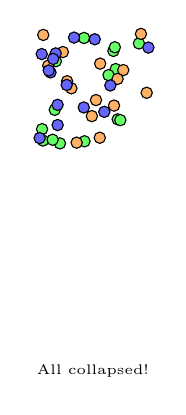
\begin{tikzpicture}[scale=1.8]
% All points compressed to center
\foreach \i in {1,...,15} {
    \pgfmathsetmacro\rx{rand*0.4}
    \pgfmathsetmacro\ry{rand*0.4}
    \draw[fill=green!60] (\rx,\ry) circle (0.04cm);
}
\foreach \i in {1,...,15} {
    \pgfmathsetmacro\rx{rand*0.4}
    \pgfmathsetmacro\ry{rand*0.4}
    \draw[fill=orange!60] (\rx,\ry) circle (0.04cm);
}
\foreach \i in {1,...,15} {
    \pgfmathsetmacro\rx{rand*0.4}
    \pgfmathsetmacro\ry{rand*0.4}
    \draw[fill=blue!60] (\rx,\ry) circle (0.04cm);
}
\node at (0,-2) {\tiny All collapsed!};
\end{tikzpicture}
\vspace{0.2cm}

\textbf{All distances collapse}\\
{\small Cannot distinguish distances}
\end{center}
\end{columns}

\vspace{0.4cm}
\begin{center}
\colorbox{red!20}{\parbox{0.9\textwidth}{\centering\textbf{The Crowding Problem:} Linear projection fails because moderate distances in high-D have no room in 2D}}
\end{center}

\footnotesize\textit{Run interactive\_demo.html to explore this yourself}
\end{frame}

% Slide 4
\begin{frame}{What You Will Master Today: A Complete Journey}
\begin{columns}
\column{0.5\textwidth}
\textbf{Conceptual Mastery}
\begin{itemize}
\item Why information $>$ distance
\item Maximum entropy emergence
\item KL divergence as design choice
\item Crowding as geometric inevitability
\end{itemize}

\textbf{Mathematical Foundation}
\begin{itemize}
\item Derive kernels from principles
\item Gradient as physical forces
\item Prove Student's t necessity
\item Understand convergence
\end{itemize}

\column{0.5\textwidth}
\textbf{Practical Excellence}
\begin{itemize}
\item Debug visually \& quantitatively
\item Choose hyperparameters wisely
\item Validate beyond visualization
\item Recognize failure modes
\end{itemize}

\textbf{Ethical Responsibility}
\begin{itemize}
\item Avoid false pattern creation
\item Communicate limitations
\item Document completely
\item Interpret responsibly
\end{itemize}
\end{columns}

\vspace{0.2cm}
\colorbox{yellow!30}{\textbf{Critical:} Mathematics and visuals will be interwoven, not separated}
\end{frame}

% Slide 5
\begin{frame}{The Paradigm Shift: From Preserving to Accepting Loss}
\begin{center}
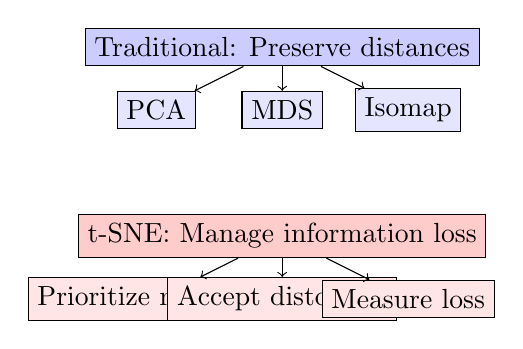
\begin{tikzpicture}[scale=0.8]
% Traditional approach
\node[rectangle, draw, fill=blue!20] (trad) at (0,3) {Traditional: Preserve distances};
\node[rectangle, draw, fill=blue!10] (pca) at (-2,2) {PCA};
\node[rectangle, draw, fill=blue!10] (mds) at (0,2) {MDS};
\node[rectangle, draw, fill=blue!10] (iso) at (2,2) {Isomap};
\draw[->] (trad) -- (pca);
\draw[->] (trad) -- (mds);
\draw[->] (trad) -- (iso);

% t-SNE approach
\node[rectangle, draw, fill=red!20] (tsne) at (0,0) {t-SNE: Manage information loss};
\node[rectangle, draw, fill=red!10] (prior) at (-2,-1) {Prioritize neighbors};
\node[rectangle, draw, fill=red!10] (accept) at (0,-1) {Accept distortion};
\node[rectangle, draw, fill=red!10] (measure) at (2,-1) {Measure loss};
\draw[->] (tsne) -- (prior);
\draw[->] (tsne) -- (accept);
\draw[->] (tsne) -- (measure);
\end{tikzpicture}
\end{center}

\intuition{t-SNE doesn't try to preserve everything - it chooses what to sacrifice}
\end{frame}

% Slide 6
\begin{frame}{Visual Intuition: The Swiss Roll Problem}
\begin{columns}
\column{0.33\textwidth}
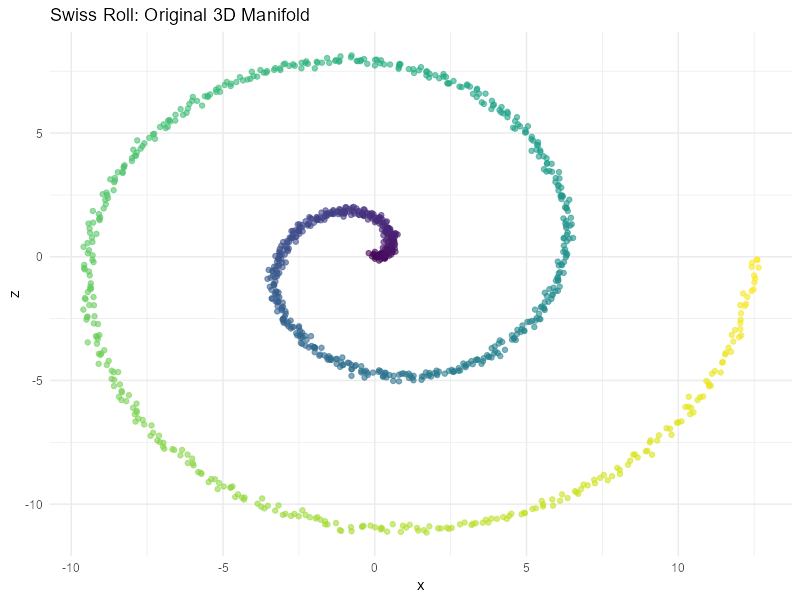
\includegraphics[width=\textwidth]{./Figures/swiss_roll_3d.png}
\textbf{Original Manifold}\\
2D surface in 3D\\
Continuous structure

\column{0.33\textwidth}
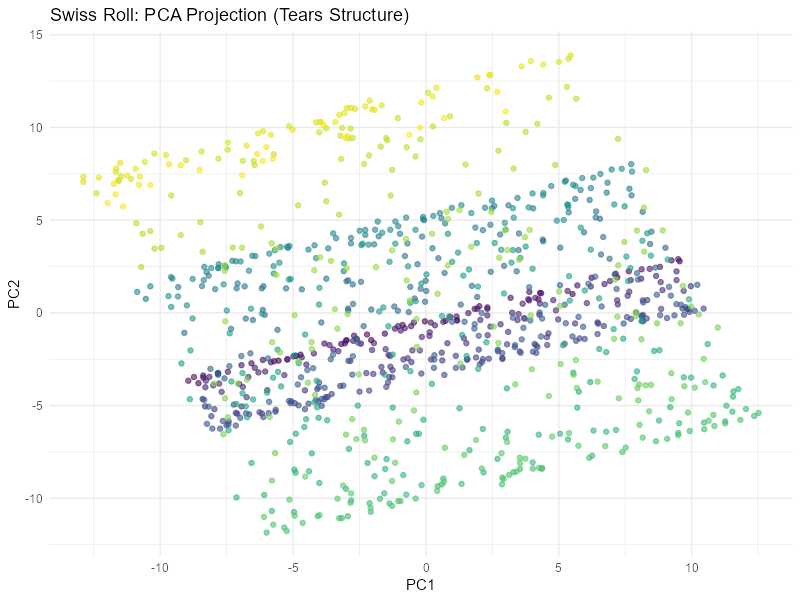
\includegraphics[width=\textwidth]{./Figures/swiss_roll_pca.png}
\textbf{PCA Projection}\\
Tears neighborhoods\\
\textcolor{red}{Destroys continuity}

\column{0.33\textwidth}
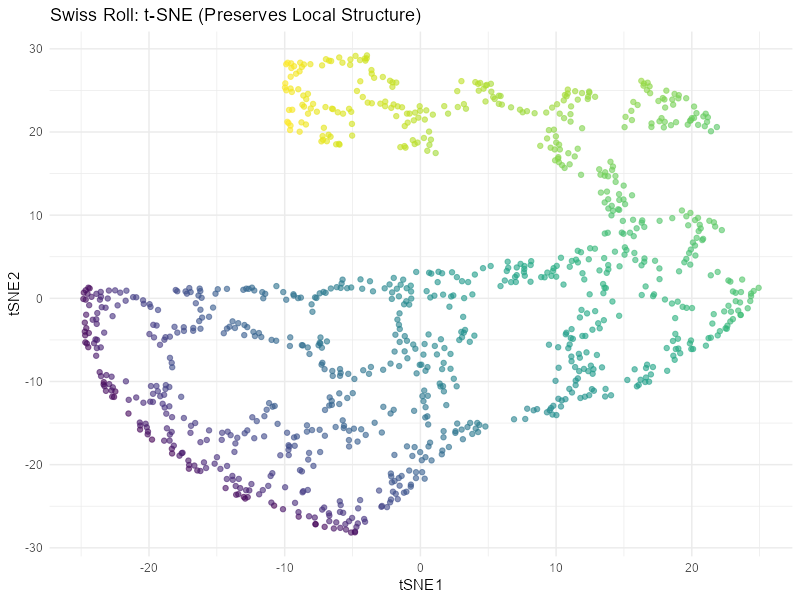
\includegraphics[width=\textwidth]{./Figures/swiss_roll_tsne.png}
\textbf{t-SNE Embedding}\\
Preserves local structure\\
\textcolor{green}{Unfolds naturally}
\end{columns}

\vspace{0.3cm}
\warning{Global structure may be sacrificed for local preservation}
\end{frame}


% Slide 7
\begin{frame}{Why Dimensionality Reduction? Real-World Impact}
\begin{center}
\begin{tikzpicture}
% Genomics
\node[draw, rectangle, minimum width=3cm, minimum height=2cm, fill=gray!20] (genomics) at (0,3) {
    \begin{tikzpicture}[scale=0.3]
    % DNA helix representation
    \foreach \i in {0,0.5,...,3} {
        \draw[blue, thick] (\i,0) sin (\i+0.25,0.3) cos (\i+0.5,0);
        \draw[red, thick] (\i,0) cos (\i+0.25,-0.3) sin (\i+0.5,0);
    }
    \foreach \i in {0,0.5,...,3} {
        \draw[gray] (\i,0.3) -- (\i,-0.3);
    }
    \end{tikzpicture}
};
\node[text width=3cm, align=center, below=0.1cm of genomics] 
    {\textbf{Genomics}\\20,000 genes\\Find disease subtypes};

% NLP
\node[draw, rectangle, minimum width=3cm, minimum height=2cm, fill=gray!20] (nlp) at (4,3) {
    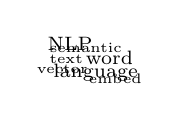
\begin{tikzpicture}[scale=0.25]
    % Word cloud representation
    \node[font=\tiny] at (0,0.8) {semantic};
    \node[font=\scriptsize] at (1.2,0.3) {word};
    \node[font=\tiny] at (-1,0.2) {text};
    \node[font=\scriptsize] at (0.5,-0.5) {language};
    \node[font=\tiny] at (-1.2,-0.3) {vector};
    \node[font=\tiny] at (1.5,-0.8) {embed};
    \node[font=\scriptsize] at (-0.8,1) {NLP};
    \end{tikzpicture}
};
\node[text width=3cm, align=center, below=0.1cm of nlp] 
    {\textbf{NLP}\\50,000 words\\Discover semantics};

% Vision
\node[draw, rectangle, minimum width=3cm, minimum height=2cm, fill=gray!20] (vision) at (8,3) {
    
\begin{tikzpicture}[scale=0.25]
    % Pixel grid representation
    \foreach \x in {0,...,5} {
        \foreach \y in {0,...,4} {
            \pgfmathsetmacro{\shade}{rnd*40+30}
            \fill[gray!\shade] (\x*0.4,\y*0.4) rectangle ++(0.35,0.35);
        }
    }
    \end{tikzpicture}
};
\node[text width=3cm, align=center, below=0.1cm of vision] 
    {\textbf{Vision}\\Million pixels\\Reveal patterns};

% Convergence arrows
\coordinate (target) at (4,0);
\draw[->, thick, red, line width=1.5pt] (genomics.south) -- (target);
\draw[->, thick, red, line width=1.5pt] (nlp.south) -- (target);
\draw[->, thick, red, line width=1.5pt] (vision.south) -- (target);

% Target label
\node[below=0.1cm] at (target) {\textbf{2D Visualization}};
\end{tikzpicture}
\end{center}

\vspace{0.3cm}
\textbf{Common Thread:} Data lives on low-dimensional manifold in high-D space
\end{frame}

% Slide 8
\begin{frame}{The Curse of Dimensionality: A Visual Catastrophe}
\begin{columns}
\column{0.5\textwidth}
\begin{center}
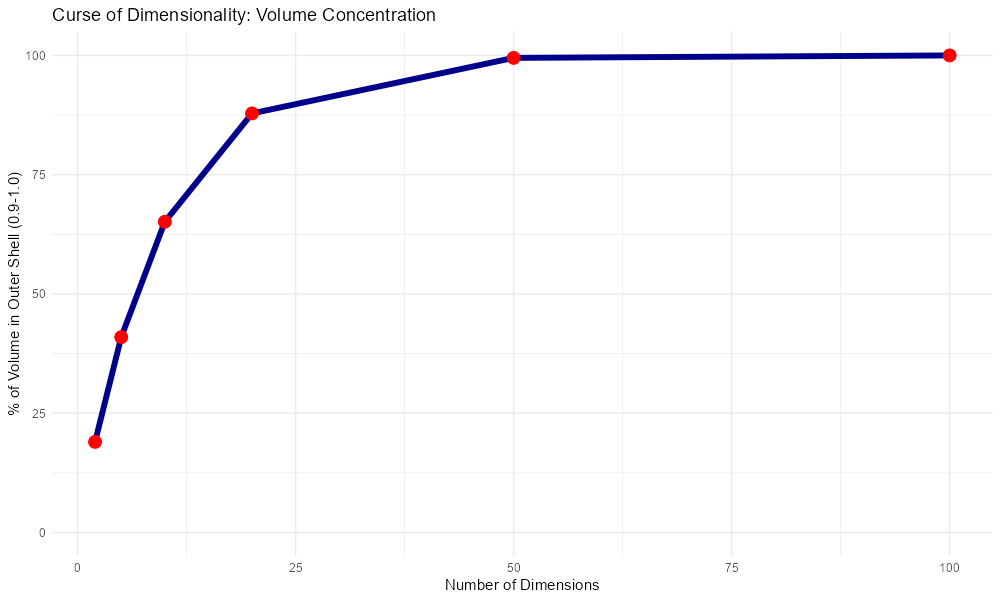
\includegraphics[width=0.9\textwidth]{./Figures/curse_dimensionality_animation.png}
\end{center}
\textbf{Volume in n-D sphere shells:}\\
\small
\begin{tabular}{l|r}
Dimension & Shell (0.9-1.0)\\
\hline
2D & 19\%\\
10D & 65\%\\
100D & 99.997\%\\
1000D & $\approx$100\%
\end{tabular}

\column{0.5\textwidth}
\textbf{Implications:}
\begin{itemize}
\item All points become equidistant
\item Nearest neighbor meaningless
\item Intuition completely fails
\item Traditional metrics break
\end{itemize}

\vspace{0.5cm}
\intuition{In high-D, everything is far from everything else, yet nothing has room}
\end{columns}
\end{frame}

% Slide 9
\begin{frame}{Reframing: From Geometry to Information Theory}
\begin{center}
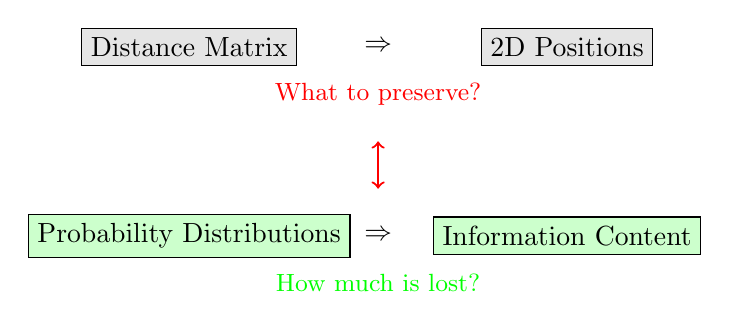
\begin{tikzpicture}[scale=1.2]
% Traditional view
\node[draw, fill=gray!20] (dist) at (0,2) {Distance Matrix};
\node (arrow1) at (2,2) {$\Rightarrow$};
\node[draw, fill=gray!20] (proj) at (4,2) {2D Positions};
\node at (2,1.5) {\textcolor{red}{\small What to preserve?}};

% Information view
\node[draw, fill=green!20] (prob) at (0,0) {Probability Distributions};
\node (arrow2) at (2,0) {$\Rightarrow$};
\node[draw, fill=green!20] (info) at (4,0) {Information Content};
\node at (2,-0.5) {\textcolor{green}{\small How much is lost?}};

\draw[<->, thick, red] (2,1) -- (2,0.5);
\end{tikzpicture}
\end{center}

\begin{block}{The Key Insight}
Instead of asking "How do we preserve distances?"\\
t-SNE asks: "How do we preserve the \textbf{information} about neighborhoods?"
\end{block}
\end{frame}

% Slide 10
\begin{frame}{Information Content: Making It Concrete}
\begin{columns}
\column{0.6\textwidth}
If point $j$ has probability $p_{j|i}$ of being $i$'s neighbor:
\begin{align}
\text{Information: } I(j) &= -\log p_{j|i} \text{ bits}\\
\text{Total entropy: } H(P_i) &= -\sum_j p_{j|i}\log p_{j|i}
\end{align}
\vspace{0.3cm}
\textbf{Example:}
\begin{itemize}
\item Certain neighbor: $p = 1 \Rightarrow I = 0$ bits
\item Likely neighbor: $p = 0.5 \Rightarrow I = 1$ bit
\item Rare neighbor: $p = 0.01 \Rightarrow I = 6.64$ bits
\end{itemize}

\column{0.4\textwidth}
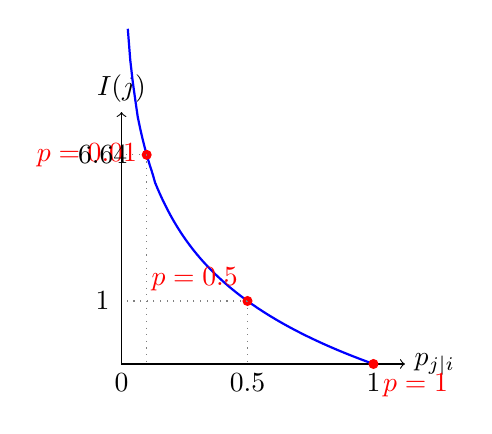
\begin{tikzpicture}[scale=0.8]
% Axes
\draw[->] (0,0) -- (4.5,0) node[right] {$p_{j|i}$};
\draw[->] (0,0) -- (0,4) node[above] {$I(j)$};

% Plot -log(p)
\draw[blue, thick, domain=0.1:4, samples=100] 
    plot (\x, {-ln(\x/4)/ln(2)});

% Mark specific points
\filldraw[red] (4, 0) circle (2pt) node[below right] {$p=1$};
\filldraw[red] (2, 1) circle (2pt) node[above left] {$p=0.5$};
\filldraw[red] (0.4, 3.32) circle (2pt) node[left] {$p=0.01$};

% Dotted lines to axes
\draw[dotted, gray] (4,0) -- (4,0);
\draw[dotted, gray] (2,1) -- (2,0);
\draw[dotted, gray] (2,1) -- (0,1);
\draw[dotted, gray] (0.4,3.32) -- (0.4,0);
\draw[dotted, gray] (0.4,3.32) -- (0,3.32);

% Axis labels
\node at (0,-0.3) {0};
\node at (2,-0.3) {0.5};
\node at (4,-0.3) {1};
\node at (-0.3,1) {1};
\node at (-0.3,3.32) {6.64};
\end{tikzpicture}

\vspace{0.2cm}
\intuition{Surprising events (unlikely neighbors) carry more information}
\end{columns}
\end{frame}

% Slide 11
\begin{frame}{From Distances to Probabilities: Visual Journey}
\begin{center}
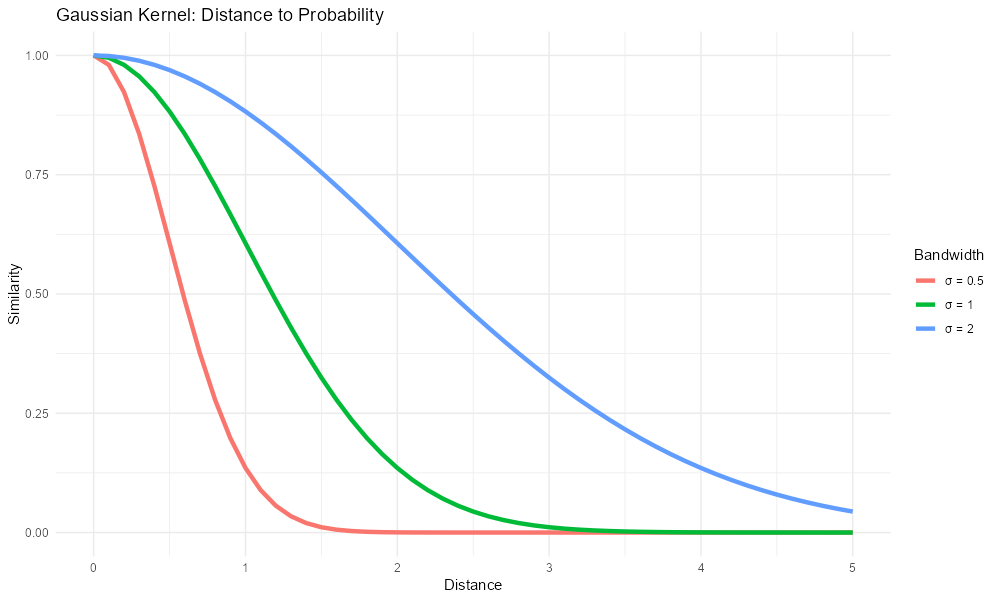
\includegraphics[width=0.9\textwidth]{./Figures/distance_to_probability_animation.png}
\end{center}

\begin{enumerate}
\item Start with distances in high-D space
\item \textbf{Problem:} Same distance means different things in dense vs sparse regions
\item \textbf{Solution:} Adaptive bandwidth Gaussian kernel
\item Convert similarities to probabilities (normalize)
\end{enumerate}

\ethics{This transformation embeds our assumptions about what matters}
\end{frame}

% Slide 12
\begin{frame}{Why Gaussian? Maximum Entropy Derivation}
\begin{block}{The Principle}
Given constraints, choose the \textbf{least biased} distribution
\end{block}

\textbf{Constraints:}
\begin{align}
\sum_j p_{j|i} &= 1 \quad \text{(probability)}\\
\sum_j p_{j|i} d_{ij}^2 &= \sigma_i^2 \quad \text{(expected squared distance)}
\end{align}

\textbf{Optimization:} Maximize $H(P_i) = -\sum_j p_{j|i}\log p_{j|i}$

\textbf{Lagrangian:}
$$\mathcal{L} = H(P_i) + \lambda\left(\sum_j p_{j|i} - 1\right) + \mu\left(\sum_j p_{j|i}d_{ij}^2 - \sigma_i^2\right)$$
\end{frame}

% Slide 13
\begin{frame}{Maximum Entropy Solution: Gaussian Emerges}
Setting $\frac{\partial\mathcal{L}}{\partial p_{j|i}} = 0$:

$$-\log p_{j|i} - 1 + \lambda + \mu d_{ij}^2 = 0$$

Solving for $p_{j|i}$:
$$p_{j|i} = \exp(\lambda - 1) \exp(-\mu d_{ij}^2)$$

After normalization:
$$p_{j|i} = \frac{\exp(-d_{ij}^2/2\sigma_i^2)}{\sum_k \exp(-d_{ik}^2/2\sigma_i^2)}$$

\begin{center}
\colorbox{yellow!30}{\textbf{The Gaussian kernel is not arbitrary - it's mathematically inevitable!}}
\end{center}

\intuition{Maximum entropy $\Rightarrow$ Make no assumptions beyond what you know}
\end{frame}

% Slide 14
\begin{frame}{Adaptive Bandwidth: The Local Density Solution}
\begin{columns}
\column{0.5\textwidth}
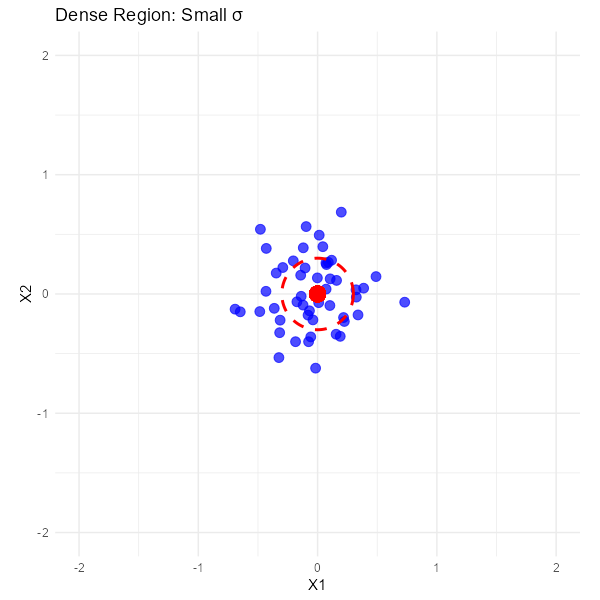
\includegraphics[width=\textwidth]{./Figures/adaptive_bandwidth_dense.png}
\textbf{Dense Region}\\
Small $\sigma_i$ captures many neighbors

\column{0.5\textwidth}
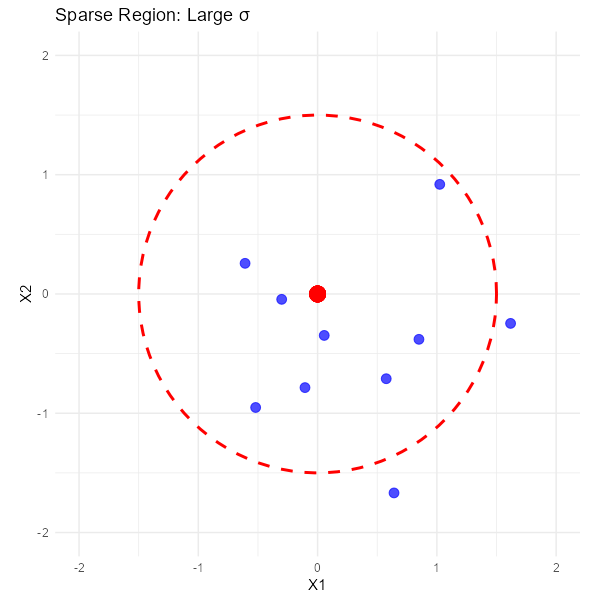
\includegraphics[width=\textwidth]{./Figures/adaptive_bandwidth_sparse.png}
\textbf{Sparse Region}\\
Large $\sigma_i$ reaches distant points
\end{columns}

\vspace{0.3cm}
\textbf{The Problem:} How to set thousands of $\sigma_i$ values?\\
\textbf{The Solution:} Perplexity - one intuitive parameter for all!

\warning{Fixed bandwidth would oversimplify dense regions or fragment sparse ones}
\end{frame}

% Slide 15
\begin{frame}{Perplexity: The Intuitive Control Parameter}
\begin{block}{Definition}
$$\text{Perp}(P_i) = 2^{H(P_i)}$$
where $H(P_i) = -\sum_j p_{j|i}\log_2 p_{j|i}$ is entropy in bits.
\end{block}

\begin{columns}
\column{0.5\textwidth}
\textbf{Interpretation:}
\begin{itemize}
\item Perp = 30 $\approx$ "30 effective neighbors"
\item Automatically adapts $\sigma_i$ per point
\item Binary search finds right $\sigma_i$
\end{itemize}

\column{0.5\textwidth}
% Change is on this next line
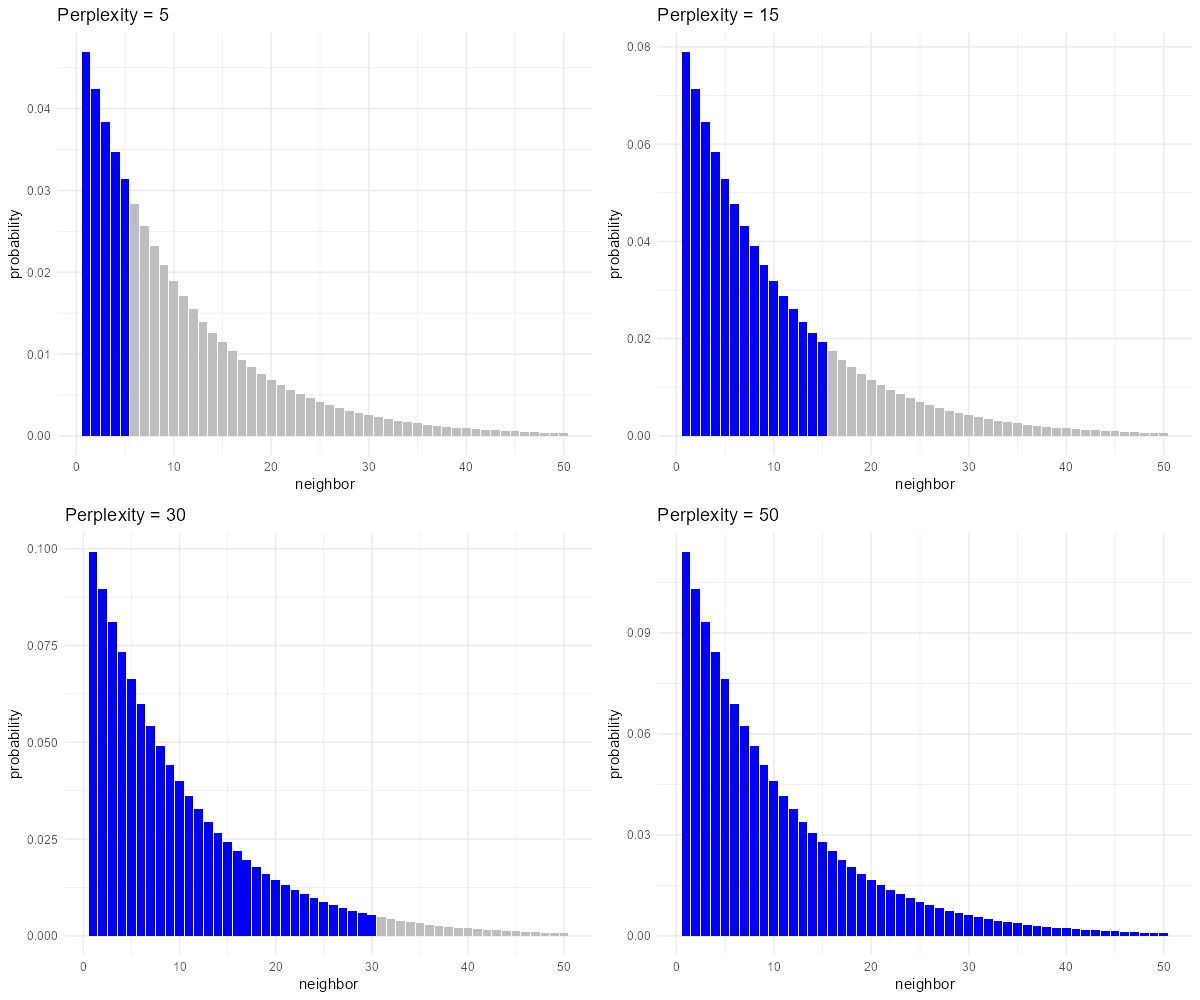
\includegraphics[width=0.7\textwidth]{./Figures/perplexity_visual.png}
\end{columns}

\intuition{Perplexity is "how many neighbors should each point care about"}
\end{frame}



% Slide 16
\begin{frame}{Algorithm: Finding $\sigma_i$ via Binary Search}
\begin{algorithm}[H]
\caption{Adaptive Bandwidth Selection}
\begin{algorithmic}[1]
\FOR{each point $i$}
\STATE target\_perp $\leftarrow$ user\_specified
\STATE $\sigma_{min} \leftarrow 0$, $\sigma_{max} \leftarrow \infty$
  \WHILE{not converged}
\STATE $\sigma_i \leftarrow (\sigma_{min} + \sigma_{max})/2$
  \STATE Compute $p_{j|i}$ using current $\sigma_i$
  \STATE current\_perp $\leftarrow 2^{H(P_i)}$
  \IF{current\_perp $>$ target\_perp}
\STATE $\sigma_{max} \leftarrow \sigma_i$ \COMMENT{Too many neighbors}
\ELSE
\STATE $\sigma_{min} \leftarrow \sigma_i$ \COMMENT{Too few neighbors}
\ENDIF
\ENDWHILE
\ENDFOR
\end{algorithmic}
\end{algorithm}
\end{frame}


% Slide 17
\begin{frame}{Measuring Information Loss: KL Divergence}
\begin{columns}
\column{0.6\textwidth}
\textbf{Cross-Entropy:} Bits using wrong distribution
$$H(P,Q) = -\sum_j p_j \log q_j$$
\textbf{KL Divergence:} Extra bits from using $Q$ instead of $P$
$$\text{KL}(P||Q) = \sum_j p_j \log\frac{p_j}{q_j}$$
\textbf{Critical Asymmetry:}
\begin{itemize}
\item Miss a neighbor: $p=0.3, q=0.01$\\
Penalty: $0.3 \log(30) \approx 1.02$ bits
\item False neighbor: $p=0.01, q=0.3$\\
Penalty: $0.01 \log(0.033) \approx -0.035$ bits
\end{itemize}
  
\column{0.4\textwidth}
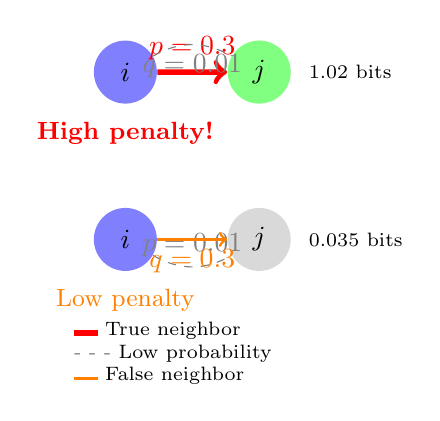
\begin{tikzpicture}[scale=0.85]
% Two scenarios visualization
% Scenario 1: Missing neighbor (high penalty)
\node[circle, fill=blue!50, minimum size=0.8cm] (p1) at (0,3) {$i$};
\node[circle, fill=green!50, minimum size=0.8cm] (q1) at (2,3) {$j$};
\draw[->, thick, red, line width=2pt] (p1) -- (q1) node[midway, above] {$p=0.3$};
\draw[dashed, gray] (p1) to[bend left=30] node[midway, below] {$q=0.01$} (q1);
\node[below=0.1cm of p1, text=red, font=\small\bfseries] {High penalty!};
\node[right=0.1cm of q1, font=\scriptsize] {1.02 bits};

% Scenario 2: False neighbor (low penalty)
\node[circle, fill=blue!50, minimum size=0.8cm] (p2) at (0,0.5) {$i$};
\node[circle, fill=gray!30, minimum size=0.8cm] (q2) at (2,0.5) {$j$};
\draw[dashed, gray] (p2) to[bend right=30] node[midway, above] {$p=0.01$} (q2);
\draw[->, thick, orange, line width=1pt] (p2) -- (q2) node[midway, below] {$q=0.3$};
\node[below=0.1cm of p2, text=orange, font=\small] {Low penalty};
\node[right=0.1cm of q2, font=\scriptsize] {0.035 bits};

% Legend
\node[font=\scriptsize, align=left, text width=3cm] at (1,-1.2) {
    \textcolor{red}{\rule{0.3cm}{2pt}} True neighbor\\
    \textcolor{gray}{- - -} Low probability\\
    \textcolor{orange}{\rule{0.3cm}{1pt}} False neighbor
};
\end{tikzpicture}

\vspace{0.3cm}
\colorbox{red!20}{\parbox{0.9\columnwidth}{\centering\textbf{t-SNE heavily penalizes\\separating true neighbors!}}}
\end{columns}
\end{frame}

% Slide 18
\begin{frame}{Visual KL Divergence: What We are Minimizing}
\begin{center}
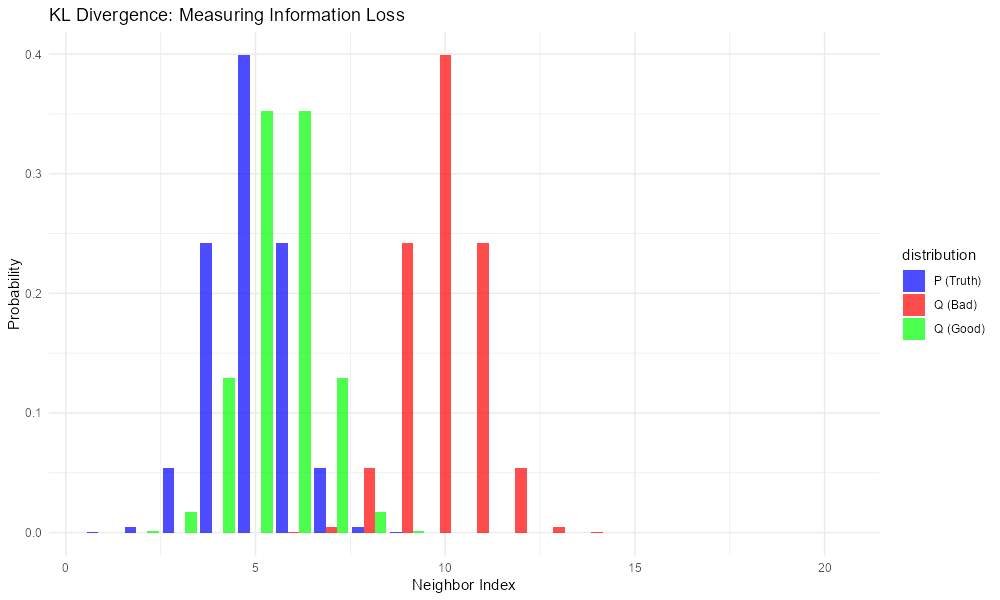
\includegraphics[width=0.5\textwidth]{./Figures/kl_divergence_visualization.png}
\end{center}
\begin{itemize}
\item \textbf{Blue bars:} High-D probability distribution $P_i$
\item \textbf{Red bars:} Low-D probability distribution $Q_i$
\item \textbf{Yellow area:} KL divergence (information lost)
\end{itemize}
\intuition{We are trying to make the red bars match the blue bars, but we care more about missing blues than extra reds}
\end{frame}


% Slide 19
  \begin{frame}{The Original SNE Algorithm}
  \begin{columns}
  \column{0.5\textwidth}
  \textbf{High-D Similarities:}
  $$p_{j|i} = \frac{\exp(-\|x_i-x_j\|^2/2\sigma_i^2)}{\sum_k \exp(-\|x_i-x_k\|^2/2\sigma_i^2)}$$
    
    \textbf{Low-D Similarities:}
  $$q_{j|i} = \frac{\exp(-\|y_i-y_j\|^2)}{\sum_k \exp(-\|y_i-y_k\|^2)}$$
    Note: Fixed variance = 1 in low-D
    
    \column{0.5\textwidth}
    \textbf{Cost Function:}
    $$C = \sum_i \text{KL}(P_i||Q_i)$$
      
      \textbf{Gradient Descent:}
    $$\frac{\partial C}{\partial y_i} = 2\sum_j (p_{j|i} - q_{j|i})(y_i - y_j)$$
      
      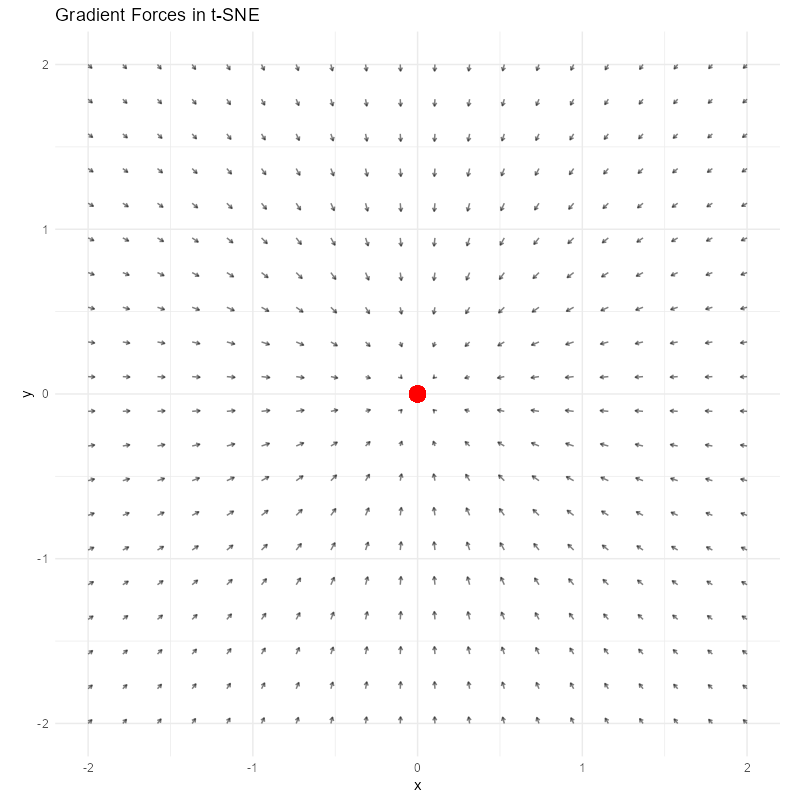
\includegraphics[width=0.5\textwidth]{./Figures/sne_gradient_forces.png}
    \end{columns}
\end{frame}
    
% Slide 20
\begin{frame}{SNE Fatal Flaw: The Crowding Problem Visualized}
\begin{center}
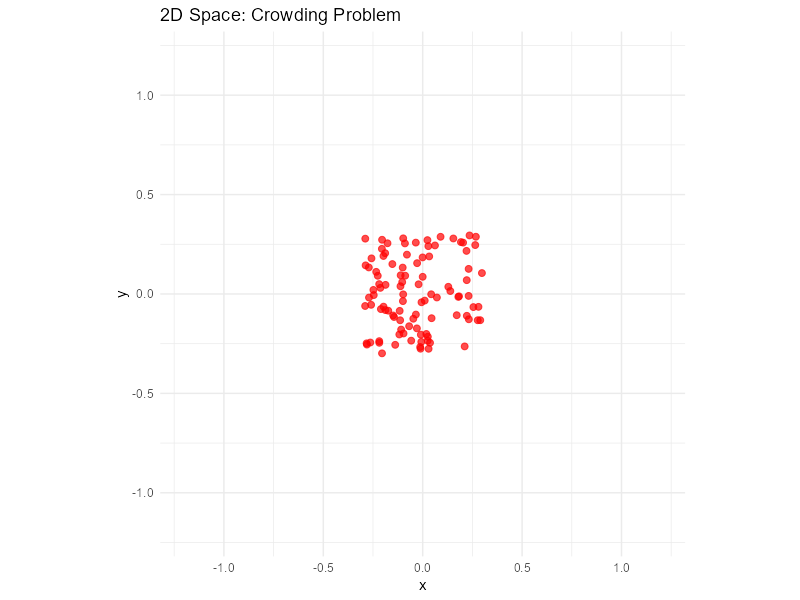
\includegraphics[width=0.3\textwidth]{./Figures/crowding_problem_animation.png}
\end{center}

\begin{columns}
\column{0.5\textwidth}
\textbf{In 10D:} Points at moderate distances\\
(0.5 - 0.8 from center)\\
Plenty of room in shell

\column{0.5\textwidth}
\textbf{In 2D:} Same distances impossible\\
Area grows as $r^2$ not $r^{10}$\\
\textcolor{red}{Moderate distances crushed!}
\end{columns}

\warning{Gaussian tails decay too fast to represent moderate distances}
\end{frame}


% Slide 21
\begin{frame}{The Brilliant Solution: Student t-Distribution}
    \begin{columns}
    \column{0.5\textwidth}
    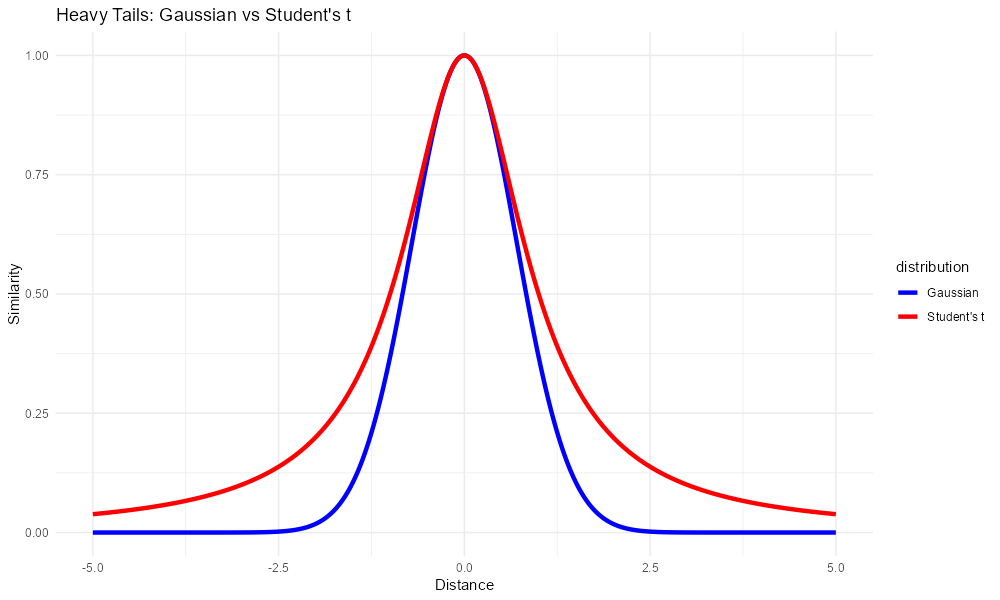
\includegraphics[width=\textwidth]{./Figures/gaussian_vs_t_comparison.png}
    
    \textbf{Mathematical Forms:}\\
    Gaussian: $\propto e^{-d^2}$\\
    Student t: $\propto (1+d^2)^{-1}$

\column{0.5\textwidth}
\textbf{Key Differences:}
\begin{itemize}
\item Polynomial vs exponential decay
\item Heavy tails = more "room"
\item Moderate distances preserved
\item Natural repulsion at distance
\end{itemize}

\intuition{Think of it as creating "virtual space" that doesnt exist in 2D}
\end{columns}

\vspace{0.3cm}
\colorbox{green!20}{\textbf{Van der Maaten \& Hinton (2008):} Use different kernels for different spaces!}
\end{frame}

% Slide 22
\begin{frame}{Why Student t? Quantitative Analysis}
\begin{columns}
\column{0.6\textwidth}
\textbf{Similarity Ratio at Different Distances:}
For $d_1 = 1$ and $d_2 = 3$:
  
  \textbf{Gaussian:}
$$\frac{q(d_1)}{q(d_2)} = \frac{e^{-1}}{e^{-9}} = e^8 \approx 2981$$
  
  \textbf{Student t:}
$$\frac{q(d_1)}{q(d_2)} = \frac{1/(1+1)}{1/(1+9)} = 5$$
  
  \column{0.4\textwidth}
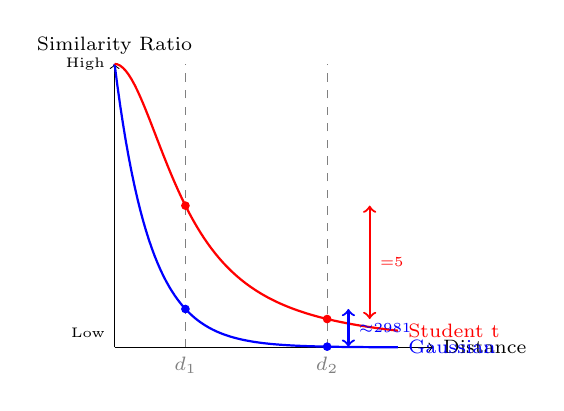
\begin{tikzpicture}[scale=0.9]
% Axes
\draw[->] (0,0) -- (4.5,0) node[right, font=\scriptsize] {Distance};
\draw[->] (0,0) -- (0,4) node[above, font=\scriptsize] {Similarity Ratio};

% Gaussian curve (exponential decay)
\draw[blue, thick, domain=0:4, samples=100] 
    plot (\x, {4*exp(-2*\x)}) node[right, font=\scriptsize] {Gaussian};

% Student t curve (polynomial decay)
\draw[red, thick, domain=0:4, samples=100] 
    plot (\x, {4/(1+\x*\x)}) node[right, font=\scriptsize] {Student t};

% Mark d1=1 and d2=3
\draw[dashed, gray] (1,0) node[below, font=\scriptsize] {$d_1$} -- (1,4);
\draw[dashed, gray] (3,0) node[below, font=\scriptsize] {$d_2$} -- (3,4);

% Mark ratios
\filldraw[blue] (1, {4*exp(-2*1)}) circle (1.5pt);
\filldraw[blue] (3, {4*exp(-2*3)}) circle (1.5pt);
\draw[<->, blue, thick] (3.3, {4*exp(-2*1)}) -- (3.3, {4*exp(-2*3)}) 
    node[midway, right, font=\tiny] {$\approx$2981};

\filldraw[red] (1, {4/(1+1*1)}) circle (1.5pt);
\filldraw[red] (3, {4/(1+3*3)}) circle (1.5pt);
\draw[<->, red, thick] (3.6, {4/(1+1*1)}) -- (3.6, {4/(1+3*3)}) 
    node[midway, right, font=\tiny] {$=$5};

% Y-axis labels
\node[left, font=\tiny] at (0,4) {High};
\node[left, font=\tiny] at (0,0.2) {Low};
\end{tikzpicture}

\vspace{0.3cm}
\colorbox{yellow!30}{\parbox{0.9\columnwidth}{\centering\textbf{600× difference in\\representation capacity!}}}
\end{columns}

\vspace{0.2cm}
\warning{This is why SNE fails - it literally runs out of space}
\end{frame}

% Slide 23
\begin{frame}{Visual Proof: How Heavy Tails Solve Crowding}
\begin{center}
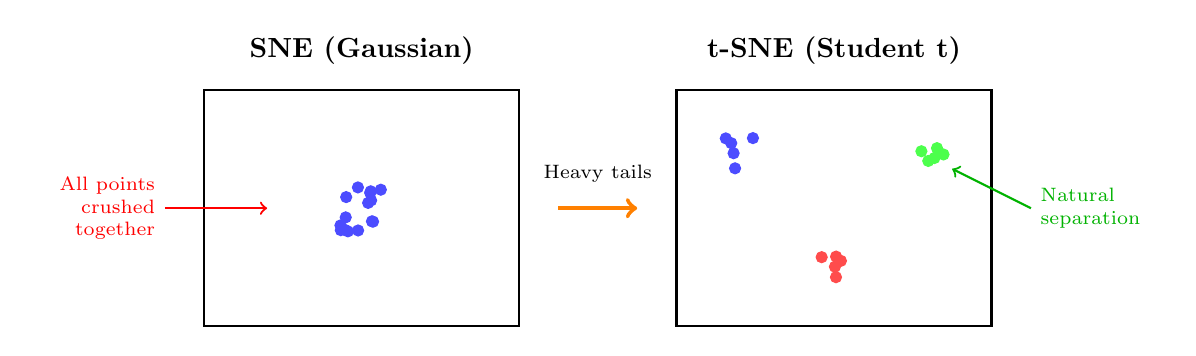
\begin{tikzpicture}[scale=1.0]
% Left side: SNE with Gaussian (crowded)
\node[font=\bfseries] at (-3,3.5) {SNE (Gaussian)};
\draw[thick] (-5,0) rectangle (-1,3);

% Central cluster - crushed together
\foreach \i in {1,...,15} {
    \pgfmathsetmacro{\x}{-3 + rand*0.3}
    \pgfmathsetmacro{\y}{1.5 + rand*0.3}
    \filldraw[blue!70] (\x,\y) circle (2pt);
}

% Annotation
\draw[->, red, thick] (-5.5,1.5) -- (-4.2,1.5);
\node[left, font=\scriptsize, text width=1.5cm, align=right, text=red] at (-5.5,1.5) 
    {All points\\crushed\\together};

% Right side: t-SNE with Student t (well-separated)
\node[font=\bfseries] at (3,3.5) {t-SNE (Student t)};
\draw[thick] (1,0) rectangle (5,3);

% Well-separated clusters
\foreach \i in {1,...,5} {
    \pgfmathsetmacro{\x}{1.8 + rand*0.2}
    \pgfmathsetmacro{\y}{2.2 + rand*0.2}
    \filldraw[blue!70] (\x,\y) circle (2pt);
}
\foreach \i in {1,...,5} {
    \pgfmathsetmacro{\x}{4.2 + rand*0.2}
    \pgfmathsetmacro{\y}{2.2 + rand*0.2}
    \filldraw[green!70] (\x,\y) circle (2pt);
}
\foreach \i in {1,...,5} {
    \pgfmathsetmacro{\x}{3 + rand*0.2}
    \pgfmathsetmacro{\y}{0.8 + rand*0.2}
    \filldraw[red!70] (\x,\y) circle (2pt);
}

% Annotation
\draw[->, green!70!black, thick] (5.5,1.5) -- (4.5,2);
\node[right, font=\scriptsize, text width=1.5cm, text=green!70!black] at (5.5,1.5) 
    {Natural\\separation};

% Central arrow showing transformation
\draw[->, ultra thick, orange] (-0.5,1.5) -- (0.5,1.5);
\node[above, font=\scriptsize] at (0,1.7) {Heavy tails};
\end{tikzpicture}
\end{center}

\vspace{0.3cm}
\begin{itemize}
\item \textbf{Left:} SNE with Gaussian - points crushed together
\item \textbf{Right:} t-SNE with Student t - natural separation
\item \textbf{Key:} Heavy tails allow moderate distances without penalty
\end{itemize}

\vspace{0.2cm}
\intuition{Heavy tails act like a "pressure valve" for crowded points}
\end{frame}


% Slide 24
\begin{frame}{The t-SNE Algorithm: Complete Specification}
\begin{block}{Key Modifications from SNE}
\begin{enumerate}
\item \textbf{Symmetrized:} $p_{ij} = \frac{p_{j|i} + p_{i|j}}{2n}$ (simplifies gradient)
\item \textbf{Student t in low-D:} $q_{ij} \propto (1 + \|y_i - y_j\|^2)^{-1}$
  \item \textbf{Single KL:} $C = \text{KL}(P||Q)$ not $\sum_i \text{KL}(P_i||Q_i)$
    \end{enumerate}
  \end{block}
  
  \textbf{Complete Cost Function:}
  $$C = \sum_{i,j} p_{ij} \log\frac{p_{ij}}{q_{ij}}$$
    
    where $q_{ij} = \frac{(1 + \|y_i - y_j\|^2)^{-1}}{\sum_{k,l} (1 + \|y_k - y_l\|^2)^{-1}}$
      \end{frame}
    
    % Slide 25
    \begin{frame}{The t-SNE Gradient: Mathematical Elegance}
    \textbf{The Gradient:}
    $$\frac{\partial C}{\partial y_i} = 4\sum_j (p_{ij} - q_{ij})(y_i - y_j)(1 + \|y_i - y_j\|^2)^{-1}$$
      
      \begin{center}
    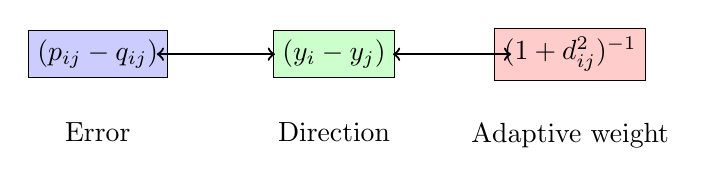
\begin{tikzpicture}[scale=1.5]
    \node[draw, fill=blue!20] (pq) at (0,0) {$(p_{ij} - q_{ij})$};
    \node[draw, fill=green!20] (dir) at (2,0) {$(y_i - y_j)$};
    \node[draw, fill=red!20] (weight) at (4,0) {$(1 + d_{ij}^2)^{-1}$};
    
    \node[below] at (0,-0.5) {Error};
    \node[below] at (2,-0.5) {Direction};
    \node[below] at (4,-0.5) {Adaptive weight};
    
    \draw[<->, thick] (0.5,0) -- (1.5,0);
    \draw[<->, thick] (2.5,0) -- (3.5,0);
    \end{tikzpicture}
    \end{center}
    
    \intuition{Forces get weaker with distance, preventing distant clusters from merging}
    \end{frame}
    
% Slide 26
\begin{frame}{Visualizing the Gradient as Forces}
\begin{center}
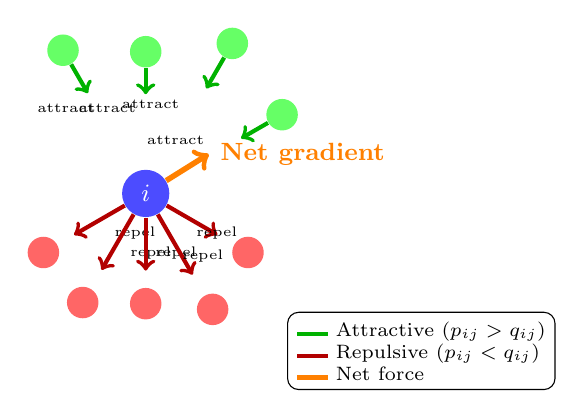
\begin{tikzpicture}[scale=1.0]
% Central reference point
\node[circle, fill=blue!70, minimum size=0.6cm, label=center:{\color{white}\small$i$}] (center) at (0,0) {};

% Attractive forces (neighbors that should be close)
\foreach \angle/\dist in {30/2, 60/2.2, 90/1.8, 120/2.1} {
    \pgfmathsetmacro{\x}{\dist*cos(\angle)}
    \pgfmathsetmacro{\y}{\dist*sin(\angle)}
    \node[circle, fill=green!60, minimum size=0.4cm] (n\angle) at (\x,\y) {};
    \draw[->, thick, green!70!black, line width=1.5pt] (n\angle) -- 
        ($(center)!0.7!(n\angle)$);
    \node[font=\tiny] at ($(n\angle)!0.5!(center)$) [above left] {attract};
}

% Repulsive forces (distant points that should stay away)
\foreach \angle/\dist in {210/1.5, 240/1.6, 270/1.4, 300/1.7, 330/1.5} {
    \pgfmathsetmacro{\x}{\dist*cos(\angle)}
    \pgfmathsetmacro{\y}{\dist*sin(\angle)}
    \node[circle, fill=red!60, minimum size=0.4cm] (n\angle) at (\x,\y) {};
    \draw[->, thick, red!70!black, line width=1.5pt] (center) -- 
        ($(n\angle)!0.3!(center)$);
    \node[font=\tiny] at ($(center)!0.4!(n\angle)$) [below right] {repel};
}

% Net force arrow on central point
\draw[->, ultra thick, orange, line width=2pt] (center) -- (0.8,0.5) 
    node[right, font=\small\bfseries] {Net gradient};

% Legend
\node[font=\scriptsize, align=left, fill=white, draw, rounded corners] at (3.5,-2) {
    \textcolor{green!70!black}{\rule{0.4cm}{1.5pt}} Attractive ($p_{ij} > q_{ij}$)\\
    \textcolor{red!70!black}{\rule{0.4cm}{1.5pt}} Repulsive ($p_{ij} < q_{ij}$)\\
    \textcolor{orange}{\rule{0.4cm}{2pt}} Net force
};
\end{tikzpicture}
\end{center}

\vspace{0.3cm}
\begin{columns}
\column{0.5\textwidth}
\textbf{Attractive Forces:}\\
When $p_{ij} > q_{ij}$\\
Pull points together\\
Preserve neighborhoods

\column{0.5\textwidth}
\textbf{Repulsive Forces:}\\
When $p_{ij} < q_{ij}$\\
Push points apart\\
Create space
\end{columns}

\vspace{0.1cm}
\ethics{The algorithm simulates physical forces - misunderstanding this leads to misinterpretation}
\end{frame}    

% Slide 27
\begin{frame}{Pseudo-code: The Core Optimization Loop}
\begin{algorithm}[H]
\caption{t-SNE Core Loop}
\begin{algorithmic}[1]
\STATE \textbf{Input:} $X \in \mathbb{R}^{n \times D}$, perplexity, T = 1000
\STATE Compute $P$ matrix using adaptive Gaussian
\STATE Symmetrize: $p_{ij} = (p_{j|i} + p_{i|j})/2n$
\STATE Initialize $Y \sim \mathcal{N}(0, 10^{-4}I)$
\FOR{$t = 1$ to $T$}
\STATE Compute $Q$ matrix using Student's t
\IF{$t < 250$} 
\STATE $P_{exag} = 4 \cdot P$ \COMMENT{Early exaggeration}
\ENDIF
\STATE $\nabla C = 4\sum_j (p_{ij} - q_{ij})(y_i - y_j)/(1 + d_{ij}^2)$
\STATE $Y^{(t)} = Y^{(t-1)} - \eta\nabla C + \alpha(Y^{(t-1)} - Y^{(t-2)})$
\STATE Adapt learning rate based on gradient sign changes
\ENDFOR
\RETURN $Y$
\end{algorithmic}
\end{algorithm}
\end{frame}

% Slide 28
\begin{frame}{Optimization Tricks: Making t-SNE Work}
\begin{columns}
\column{0.5\textwidth}
\textbf{1. Early Exaggeration}

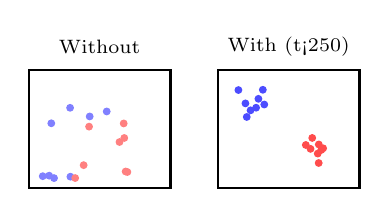
\begin{tikzpicture}[scale=0.6]
% Before early exaggeration
\begin{scope}[xshift=0cm]
\node at (0,2.5) {\scriptsize Without};
\draw[thick] (-1.5,-0.5) rectangle (1.5,2);
\foreach \i in {1,...,8} {
    \pgfmathsetmacro{\x}{-0.5 + rand*0.8}
    \pgfmathsetmacro{\y}{0.5 + rand*0.8}
    \filldraw[blue!50] (\x,\y) circle (2pt);
}
\foreach \i in {1,...,8} {
    \pgfmathsetmacro{\x}{0.2 + rand*0.8}
    \pgfmathsetmacro{\y}{0.3 + rand*0.8}
    \filldraw[red!50] (\x,\y) circle (2pt);
}
\end{scope}

% After early exaggeration
\begin{scope}[xshift=4cm]
\node at (0,2.5) {\scriptsize With (t<250)};
\draw[thick] (-1.5,-0.5) rectangle (1.5,2);
\foreach \i in {1,...,8} {
    \pgfmathsetmacro{\x}{-0.8 + rand*0.3}
    \pgfmathsetmacro{\y}{1.3 + rand*0.3}
    \filldraw[blue!70] (\x,\y) circle (2pt);
}
\foreach \i in {1,...,8} {
    \pgfmathsetmacro{\x}{0.6 + rand*0.3}
    \pgfmathsetmacro{\y}{0.3 + rand*0.3}
    \filldraw[red!70] (\x,\y) circle (2pt);
}
\end{scope}
\end{tikzpicture}

Multiply $P$ by 4 for first 250 iterations\\
Forms tight clusters early

\column{0.5\textwidth}
\textbf{2. Momentum Schedule}

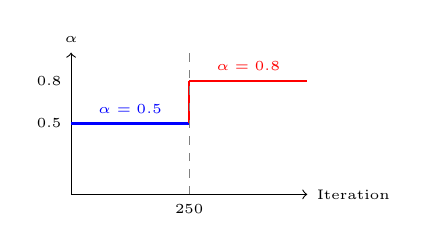
\begin{tikzpicture}[scale=0.6]
\draw[->] (0,0) -- (5,0) node[right, font=\tiny] {Iteration};
\draw[->] (0,0) -- (0,3) node[above, font=\tiny] {$\alpha$};

% Momentum schedule
\draw[thick, blue] (0,1.5) -- (2.5,1.5) node[midway, above, font=\tiny] {$\alpha=0.5$};
\draw[thick, red] (2.5,1.5) -- (2.5,2.4);
\draw[thick, red] (2.5,2.4) -- (5,2.4) node[midway, above, font=\tiny] {$\alpha=0.8$};

% Mark iteration 250
\draw[dashed, gray] (2.5,0) -- (2.5,3);
\node[below, font=\tiny] at (2.5,0) {250};

% Axis labels
\node[left, font=\tiny] at (0,1.5) {0.5};
\node[left, font=\tiny] at (0,2.4) {0.8};
\end{tikzpicture}

$\alpha = 0.5 \to 0.8$ at iteration 250\\
Escapes local minima
\end{columns}

\vspace{0.3cm}
\textbf{3. Adaptive Learning Rate:}
If gradient keeps same sign: $\eta \times 1.2$\\
If gradient changes sign: $\eta \times 0.8$

\intuition{These tricks reduce runtime from hours to minutes!}
\end{frame}

% Slide 29
\begin{frame}{Numerical Stability: Critical Implementation Details}
\begin{block}{Common Numerical Issues and Solutions}
\begin{enumerate}
\item \textbf{Log of zero:} Add $\epsilon = 10^{-12}$ to all probabilities
\item \textbf{Exponential overflow:} Use log-sum-exp trick:
$$\log\sum_i e^{x_i} = \max(x) + \log\sum_i e^{x_i - \max(x)}$$
\item \textbf{Division by zero:} Add $\epsilon$ to all squared distances
\item \textbf{Gradient explosion:} Clip if $\|\nabla\| > 100$
\item \textbf{Duplicate points:} Add small noise or remove
\end{enumerate}
\end{block}

\warning{Ignoring these causes NaN values and crashes!}

\textbf{Memory Optimization:} Use sparse $P$ matrix (only k-NN stored)
\end{frame}

% Slide 30
\begin{frame}{Barnes-Hut Approximation: From $O(n^2)$ to $O(n\log n)$}
\begin{columns}
\column{0.5\textwidth}
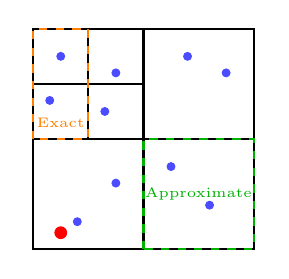
\begin{tikzpicture}[scale=0.7]
% Quadtree structure
\draw[thick] (0,0) rectangle (4,4);
\draw[thick] (2,0) -- (2,4);
\draw[thick] (0,2) -- (4,2);
\draw[thick] (1,2) -- (1,4);
\draw[thick] (0,3) -- (2,3);

% Points
\foreach \x/\y in {0.5/3.5, 0.3/2.7, 1.5/3.2, 1.3/2.5, 2.8/3.5, 3.5/3.2, 2.5/1.5, 3.2/0.8, 0.8/0.5, 1.5/1.2} {
    \filldraw[blue!70] (\x,\y) circle (2pt);
}

% Highlight one query point
\filldraw[red] (0.5,0.3) circle (3pt);

% Show approximation regions
\draw[dashed, green!70!black, thick] (2,0) rectangle (4,2);
\node[green!70!black, font=\tiny] at (3,1) {Approximate};

\draw[dashed, orange, thick] (0,2) rectangle (1,4);
\node[orange, font=\tiny] at (0.5,2.3) {Exact};
\end{tikzpicture}

\textbf{Key Idea:}\\
Treat distant point clusters as single mass

\column{0.5\textwidth}
\textbf{Criterion:}
$$\frac{r_{cell}}{d_{to\_cell}} < \theta$$

\begin{itemize}
\item $\theta = 0$: Exact (slow)
\item $\theta = 0.5$: Good balance
\item $\theta = 1$: Fast (inaccurate)
\end{itemize}

\textbf{Speedup:}\\
10K points: 50× faster\\
100K points: 200× faster
\end{columns}

\vspace{0.2cm}
\intuition{Most computation is repulsive forces between distant points - approximate them!}
\end{frame}

% Slide 31
\begin{frame}{Debugging t-SNE: Visual Diagnosis Guide}
\begin{center}
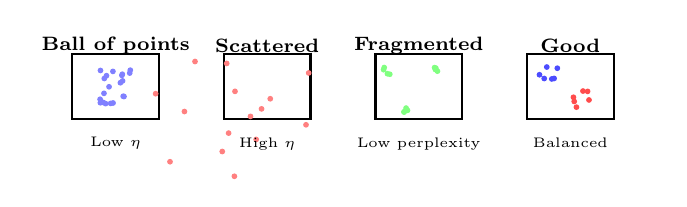
\begin{tikzpicture}[scale=0.55]
% Ball of points
\node at (0,3.2) {\scriptsize\textbf{Ball of points}};
\draw[thick] (-1,1.5) rectangle (1,3);
\foreach \i in {1,...,20} {
    \pgfmathsetmacro{\x}{rand*0.4}
    \pgfmathsetmacro{\y}{2.25 + rand*0.4}
    \filldraw[blue!50] (\x,\y) circle (1.5pt);
}
\node[below, font=\tiny, text width=2cm, align=center] at (0,1.3) {Low $\eta$};

% Scattered points
\node at (3.5,3.2) {\scriptsize\textbf{Scattered}};
\draw[thick] (2.5,1.5) rectangle (4.5,3);
\foreach \i in {1,...,15} {
    \pgfmathsetmacro{\x}{2.5 + rand*2}
    \pgfmathsetmacro{\y}{1.5 + rand*1.5}
    \filldraw[red!50] (\x,\y) circle (1.5pt);
}
\node[below, font=\tiny, text width=2cm, align=center] at (3.5,1.3) {High $\eta$};

% Fragmented clusters
\node at (7,3.2) {\scriptsize\textbf{Fragmented}};
\draw[thick] (6,1.5) rectangle (8,3);
\foreach \i in {1,...,4} {
    \pgfmathsetmacro{\x}{6.3 + rand*0.15}
    \pgfmathsetmacro{\y}{2.6 + rand*0.15}
    \filldraw[green!50] (\x,\y) circle (1.5pt);
}
\foreach \i in {1,...,4} {
    \pgfmathsetmacro{\x}{7.5 + rand*0.15}
    \pgfmathsetmacro{\y}{2.6 + rand*0.15}
    \filldraw[green!50] (\x,\y) circle (1.5pt);
}
\foreach \i in {1,...,4} {
    \pgfmathsetmacro{\x}{6.8 + rand*0.15}
    \pgfmathsetmacro{\y}{1.8 + rand*0.15}
    \filldraw[green!50] (\x,\y) circle (1.5pt);
}
\node[below, font=\tiny, text width=2cm, align=center] at (7,1.3) {Low perplexity};

% Good result
\node at (10.5,3.2) {\scriptsize\textbf{Good}};
\draw[thick] (9.5,1.5) rectangle (11.5,3);
\foreach \i in {1,...,6} {
    \pgfmathsetmacro{\x}{10 + rand*0.25}
    \pgfmathsetmacro{\y}{2.5 + rand*0.25}
    \filldraw[blue!70] (\x,\y) circle (1.5pt);
}
\foreach \i in {1,...,6} {
    \pgfmathsetmacro{\x}{10.8 + rand*0.25}
    \pgfmathsetmacro{\y}{1.9 + rand*0.25}
    \filldraw[red!70] (\x,\y) circle (1.5pt);
}
\node[below, font=\tiny, text width=2cm, align=center] at (10.5,1.3) {Balanced};
\end{tikzpicture}
\end{center}

\vspace{0.3cm}
\begin{tabular}{l|l|l}
\textbf{Symptom} & \textbf{Cause} & \textbf{Fix}\\
\hline
Ball of points & Learning rate too low & Increase $\eta$\\
Scattered points & Learning rate too high & Decrease $\eta$\\
Fragmented clusters & Perplexity too low & Increase perplexity\\
No structure & Too few iterations & Increase T\\
Different each run & Not converged & More iterations
\end{tabular}

\vspace{0.2cm}
\ethics{Always run multiple times - single runs can be misleading!}
\end{frame}

% Slide 32
\begin{frame}{Perplexity Deep Dive: Your Main Control}
\begin{center}
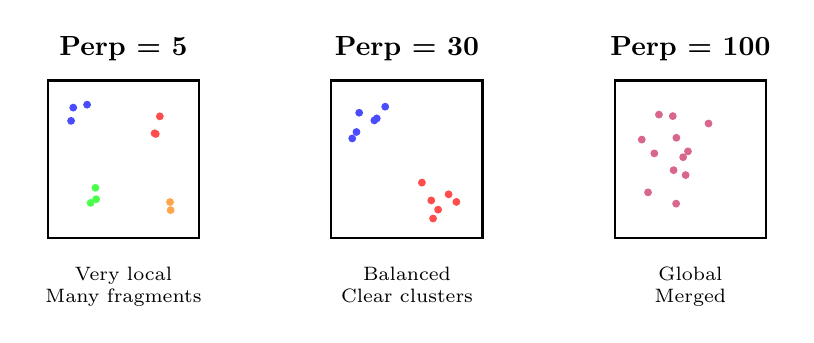
\begin{tikzpicture}[scale=0.8]
% Perplexity = 5
\begin{scope}[xshift=0cm]
\node at (0,3) {\textbf{Perp = 5}};
\draw[thick] (-1.2,0) rectangle (1.2,2.5);
\foreach \i in {1,...,3} {
    \pgfmathsetmacro{\x}{-0.7 + rand*0.15}
    \pgfmathsetmacro{\y}{2 + rand*0.15}
    \filldraw[blue!70] (\x,\y) circle (1.5pt);
}
\foreach \i in {1,...,3} {
    \pgfmathsetmacro{\x}{0.6 + rand*0.15}
    \pgfmathsetmacro{\y}{1.8 + rand*0.15}
    \filldraw[red!70] (\x,\y) circle (1.5pt);
}
\foreach \i in {1,...,3} {
    \pgfmathsetmacro{\x}{-0.5 + rand*0.15}
    \pgfmathsetmacro{\y}{0.7 + rand*0.15}
    \filldraw[green!70] (\x,\y) circle (1.5pt);
}
\foreach \i in {1,...,2} {
    \pgfmathsetmacro{\x}{0.7 + rand*0.1}
    \pgfmathsetmacro{\y}{0.5 + rand*0.1}
    \filldraw[orange!70] (\x,\y) circle (1.5pt);
}
\node[below, font=\scriptsize, text width=2.2cm, align=center] at (0,-0.3) {Very local\\Many fragments};
\end{scope}

% Perplexity = 30
\begin{scope}[xshift=4.5cm]
\node at (0,3) {\textbf{Perp = 30}};
\draw[thick] (-1.2,0) rectangle (1.2,2.5);
\foreach \i in {1,...,6} {
    \pgfmathsetmacro{\x}{-0.6 + rand*0.3}
    \pgfmathsetmacro{\y}{1.8 + rand*0.3}
    \filldraw[blue!70] (\x,\y) circle (1.5pt);
}
\foreach \i in {1,...,6} {
    \pgfmathsetmacro{\x}{0.5 + rand*0.3}
    \pgfmathsetmacro{\y}{0.6 + rand*0.3}
    \filldraw[red!70] (\x,\y) circle (1.5pt);
}
\node[below, font=\scriptsize, text width=2.2cm, align=center] at (0,-0.3) {Balanced\\Clear clusters};
\end{scope}

% Perplexity = 100
\begin{scope}[xshift=9cm]
\node at (0,3) {\textbf{Perp = 100}};
\draw[thick] (-1.2,0) rectangle (1.2,2.5);
\foreach \i in {1,...,12} {
    \pgfmathsetmacro{\x}{-0.3 + rand*0.6}
    \pgfmathsetmacro{\y}{1.25 + rand*0.8}
    \filldraw[purple!60] (\x,\y) circle (1.5pt);
}
\node[below, font=\scriptsize, text width=2.2cm, align=center] at (0,-0.3) {Global\\Merged};
\end{scope}
\end{tikzpicture}
\end{center}

\vspace{0.3cm}
\begin{columns}
\column{0.33\textwidth}
\textbf{Perp = 5}\\
Very local focus\\
Many fragments\\
Good for outliers

\column{0.33\textwidth}
\textbf{Perp = 30}\\
Balanced view\\
Clear clusters\\
Most common choice

\column{0.33\textwidth}
\textbf{Perp = 100}\\
Global structure\\
Merges clusters\\
Loses detail
\end{columns}

\vspace{0.2cm}
\warning{Truth is what's consistent across multiple perplexity values}
\end{frame}

% Slide 33
\begin{frame}{Critical: What You CANNOT Interpret}
\begin{center}
\colorbox{red!30}{\Large\textbf{The Three Deadly Sins of t-SNE Interpretation}}
\end{center}

\begin{columns}
\column{0.33\textwidth}
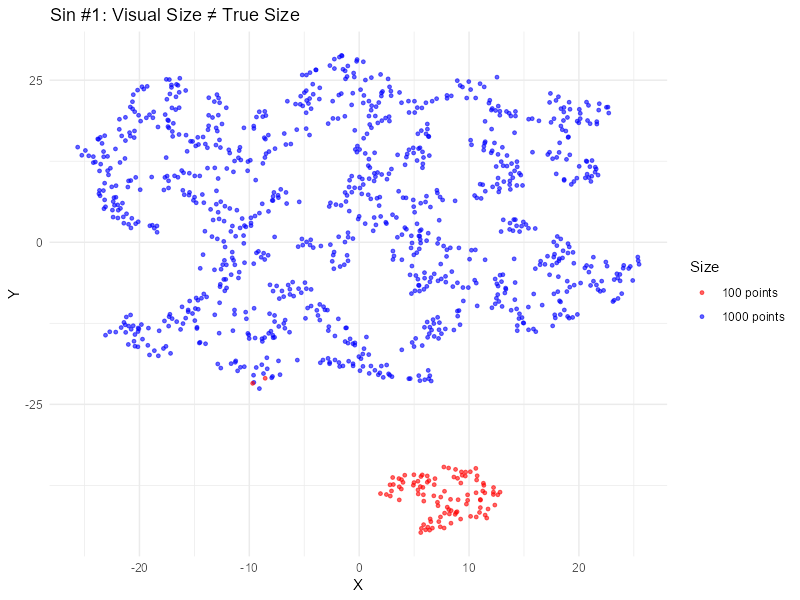
\includegraphics[width=\textwidth]{./Figures/sin1_cluster_size.png}
\textbf{Sin \#1: Cluster Sizes}\\
  1000 vs 100 points\\
  Look same size!
    
    \column{0.33\textwidth}
  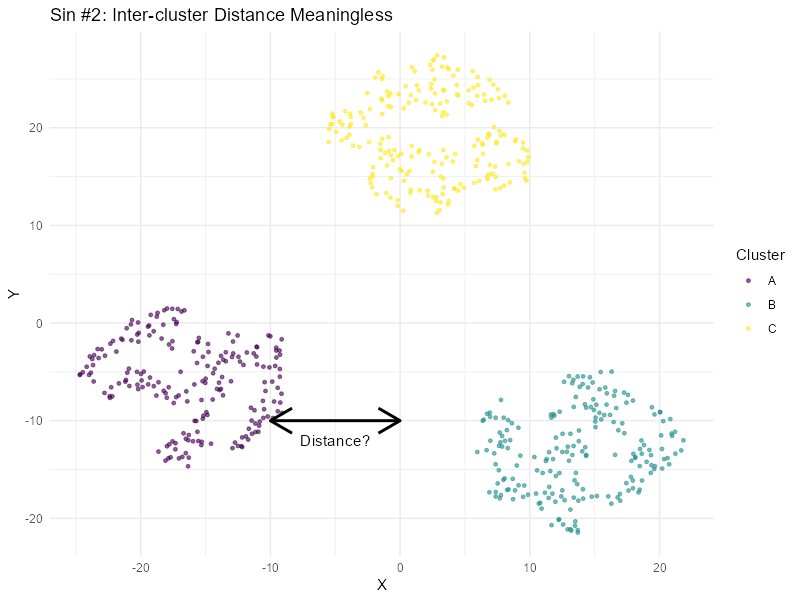
\includegraphics[width=\textwidth]{./Figures/sin2_distances.png}
  \textbf{Sin \#2: Inter-cluster Distance}\\
    Gap size meaningless\\
    No global coordinates
    
    \column{0.33\textwidth}
    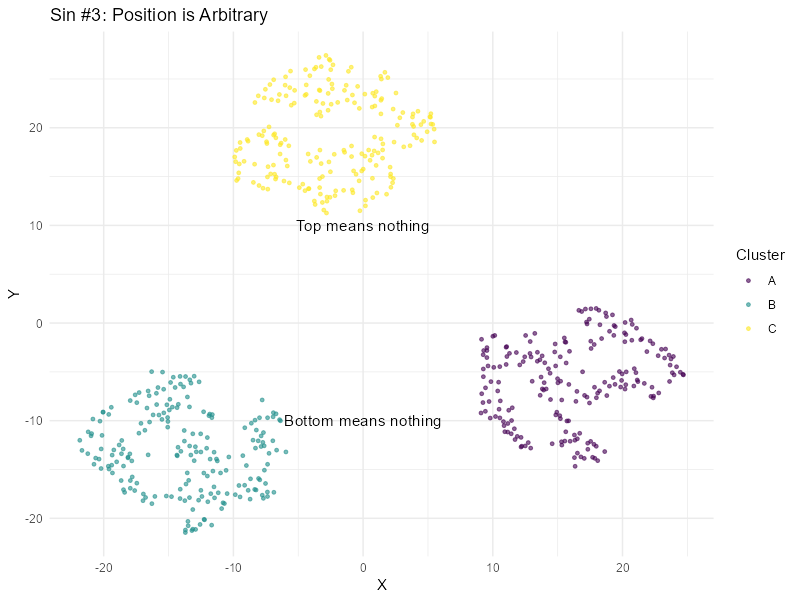
\includegraphics[width=\textwidth]{./Figures/sin3_position.png}
    \textbf{Sin \#3: Absolute Position}\\
      Top vs bottom\\
      Rotation arbitrary
      \end{columns}
      
      \vspace{0.3cm}
      \colorbox{green!30}{\textbf{What you CAN trust:} Local neighborhoods and cluster separation}
      \end{frame}
      
      % Slide 34
      \begin{frame}{Case Study: MNIST Digits - Complete Pipeline}
      \begin{columns}
      \column{0.5\textwidth}
      \textbf{Data:}
      \begin{itemize}
      \item 70,000 handwritten digits
      \item $28×28 = 784$ dimensions
      \item 10 classes (0-9)
      \end{itemize}
      
      \textbf{Pipeline:}
      \begin{enumerate}
      \item Scale pixels to [0,1]
      \item PCA to 50D (95\% variance)
      \item Remove outliers ($>$ 3$\sigma$)
      \item t-SNE with perp $=30$
      \item Validate with NPr metric
      \end{enumerate}
      
      \column{0.5\textwidth}
      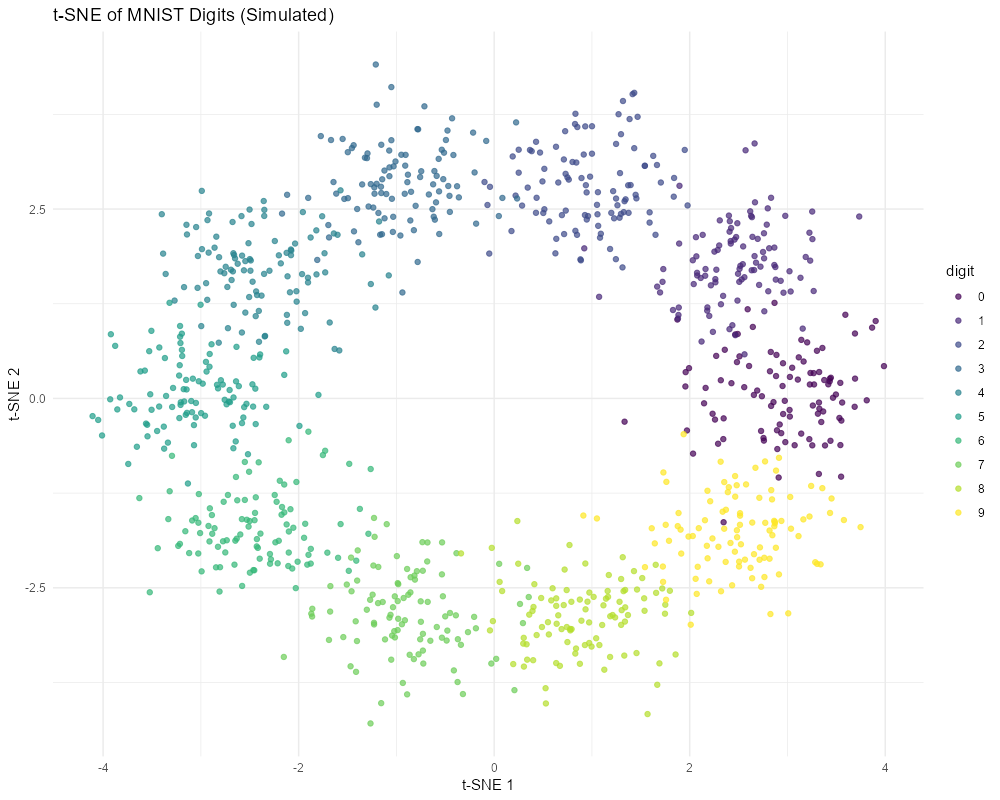
\includegraphics[width=0.8\textwidth]{./Figures/mnist_tsne_result.png}
      
      \textbf{Observations:}
      \begin{itemize}
      \item Clear digit separation
      \item 4-9 proximity (visual similarity)
      \item Sub-clusters = writing styles
      \end{itemize}
      \end{columns}
      
      \textit{Run tsne\_mnist.R for full analysis}
      \end{frame}


% Slide 35
\begin{frame}{Validation: Beyond Visual Inspection}
\begin{columns}
\column{0.55\textwidth}
\begin{block}{Quantitative Validation Metrics}
\textbf{1. Neighborhood Preservation (NPr):}
$$\text{NPr}(k) = \frac{1}{n}\sum_i \frac{|N_k^{high}(i) \cap N_k^{low}(i)|}{k}$$
  
\textbf{2. Trustworthiness:}
$$T(k) = 1 - \frac{2}{nk(2n-3k-1)}\sum_i \sum_{j \in U_k(i)} (r(i,j) - k)$$
  
\textbf{3. Continuity:}
$$C(k) = 1 - \frac{2}{nk(2n-3k-1)}\sum_i \sum_{j \in V_k(i)} (r'(i,j) - k)$$
\end{block}

\column{0.45\textwidth}
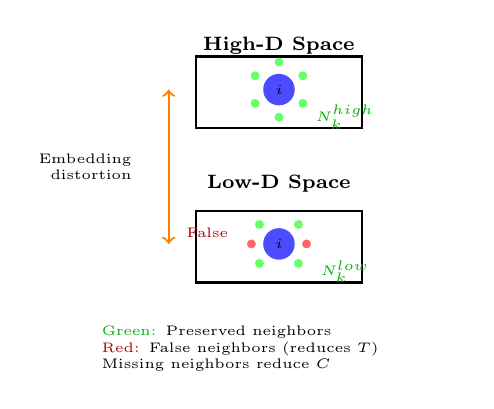
\begin{tikzpicture}[scale=0.7]
% High-dimensional space
\node at (0,5) {\scriptsize\textbf{High-D Space}};
\draw[thick] (-1.5,3.5) rectangle (1.5,4.8);
\node[circle, fill=blue!70, minimum size=0.4cm, label=center:{\tiny$i$}] (hi) at (0,4.2) {};
\foreach \angle in {30,90,150,210,270,330} {
    \pgfmathsetmacro{\x}{0.5*cos(\angle)}
    \pgfmathsetmacro{\y}{4.2+0.5*sin(\angle)}
    \filldraw[green!60] (\x,\y) circle (2pt);
}
\node[font=\tiny, green!70!black] at (1.2,3.7) {$N_k^{high}$};

% Low-dimensional space
\node at (0,2.5) {\scriptsize\textbf{Low-D Space}};
\draw[thick] (-1.5,0.7) rectangle (1.5,2);
\node[circle, fill=blue!70, minimum size=0.4cm, label=center:{\tiny$i$}] (lo) at (0,1.4) {};
\foreach \angle in {45,135,225,315} {
    \pgfmathsetmacro{\x}{0.5*cos(\angle)}
    \pgfmathsetmacro{\y}{1.4+0.5*sin(\angle)}
    \filldraw[green!60] (\x,\y) circle (2pt);
}
\foreach \angle in {0,180} {
    \pgfmathsetmacro{\x}{0.5*cos(\angle)}
    \pgfmathsetmacro{\y}{1.4+0.5*sin(\angle)}
    \filldraw[red!60] (\x,\y) circle (2pt);
}
\node[font=\tiny, green!70!black] at (1.2,0.9) {$N_k^{low}$};
\node[font=\tiny, red!70!black] at (-1.3,1.6) {False};

% Annotations
\draw[<->, thick, orange] (-2,4.2) -- (-2,1.4);
\node[left, font=\tiny, text width=1.2cm, align=right] at (-2.5,2.8) {Embedding\\distortion};

% Metric interpretations
\node[font=\tiny, text width=4.5cm, align=left] at (0,-0.5) {
    \textcolor{green!70!black}{Green:} Preserved neighbors\\
    \textcolor{red!70!black}{Red:} False neighbors (reduces $T$)\\
    Missing neighbors reduce $C$
};
\end{tikzpicture}
\end{columns}

\vspace{0.3cm}
\warning{Never publish t-SNE without these metrics!}
\end{frame}

% Slide 36
\begin{frame}{Stability Analysis: How Reliable Is Your Embedding?}
\begin{columns}
\column{0.5\textwidth}
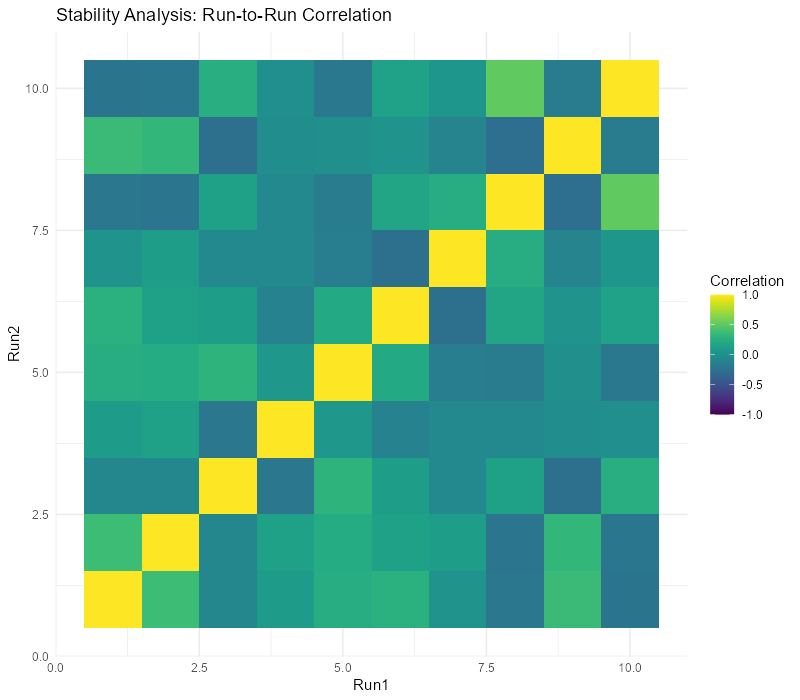
\includegraphics[width=0.5\textwidth]{./Figures/stability_analysis.png}

\textbf{Protocol:}
\begin{enumerate}
\item Run t-SNE 10 times
\item Different random seeds
\item Compute pairwise correlations
\item Report mean ± std
\end{enumerate}

\column{0.5\textwidth}
\textbf{Interpretation:}
\begin{itemize}
\item $r > 0.9$: Very stable
\item $r = 0.7-0.9$: Moderately stable
\item $r < 0.7$: Unreliable
\end{itemize}

\textbf{Causes of Instability:}
\begin{itemize}
\item Too few iterations
\item Wrong perplexity
\item Intrinsic data ambiguity
\end{itemize}
\end{columns}

\intuition{If results change dramatically between runs, dont trust them!}
\end{frame}

% Slide 37
\begin{frame}{Interactive t-SNE: Beyond Static Plots}
\begin{center}
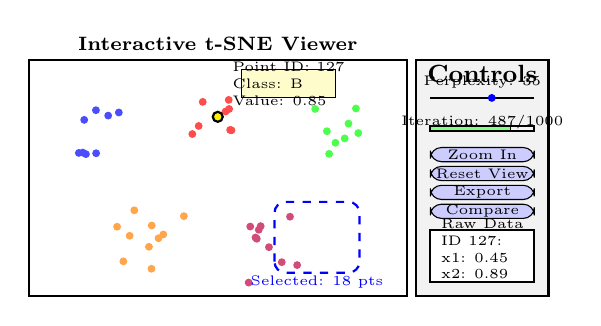
\begin{tikzpicture}[scale=0.6]
% Main visualization window
\draw[thick, fill=white] (0,0) rectangle (8,5);
\node[above] at (4,5) {\scriptsize\textbf{Interactive t-SNE Viewer}};

% Scatter plot with colored clusters
\foreach \i in {1,...,8} {
    \pgfmathsetmacro{\x}{1.5 + rand*0.5}
    \pgfmathsetmacro{\y}{3.5 + rand*0.5}
    \filldraw[blue!70] (\x,\y) circle (2pt);
}
\foreach \i in {1,...,8} {
    \pgfmathsetmacro{\x}{4 + rand*0.6}
    \pgfmathsetmacro{\y}{3.8 + rand*0.5}
    \filldraw[red!70] (\x,\y) circle (2pt);
}
\foreach \i in {1,...,8} {
    \pgfmathsetmacro{\x}{6.5 + rand*0.5}
    \pgfmathsetmacro{\y}{3.5 + rand*0.5}
    \filldraw[green!70] (\x,\y) circle (2pt);
}
\foreach \i in {1,...,10} {
    \pgfmathsetmacro{\x}{2.5 + rand*0.8}
    \pgfmathsetmacro{\y}{1.2 + rand*0.7}
    \filldraw[orange!70] (\x,\y) circle (2pt);
}
\foreach \i in {1,...,10} {
    \pgfmathsetmacro{\x}{5.5 + rand*0.9}
    \pgfmathsetmacro{\y}{1 + rand*0.8}
    \filldraw[purple!70] (\x,\y) circle (2pt);
}

% Highlight one point with hover tooltip
\filldraw[yellow, draw=black, thick] (4,3.8) circle (3pt);
\draw[fill=yellow!20, draw=black] (4.5,4.2) rectangle (6.5,4.8);
\node[font=\tiny, align=left] at (5.5,4.5) {Point ID: 127\\Class: B\\Value: 0.85};

% Selection brush
\draw[dashed, blue, thick, rounded corners] (5.2,0.5) rectangle (7,2);
\node[font=\tiny, blue] at (6.1,0.3) {Selected: 18 pts};

% Control panel on right
\draw[thick, fill=gray!10] (8.2,0) rectangle (11,5);
\node[font=\small\bfseries] at (9.6,4.7) {Controls};

% Perplexity slider
\draw[thick] (8.5,4.2) -- (10.7,4.2);
\filldraw[blue] (9.8,4.2) circle (2pt);
\node[font=\tiny, above] at (9.6,4.2) {Perplexity: 35};

% Iteration counter
\node[font=\tiny, align=left] at (9.6,3.7) {Iteration: 487/1000};
\draw[fill=green!50] (8.5,3.5) rectangle (10.2,3.6);
\draw[thick] (8.5,3.5) rectangle (10.7,3.6);

% Buttons
\foreach \y/\label in {3/Zoom In, 2.6/Reset View, 2.2/Export, 1.8/Compare} {
    \draw[fill=blue!20, rounded corners] (8.5,\y-0.15) rectangle (10.7,\y+0.15);
    \node[font=\tiny] at (9.6,\y) {\label};
}

% Linked data view
\draw[thick, fill=white] (8.5,0.3) rectangle (10.7,1.4);
\node[font=\tiny, align=left] at (9.6,1) {Raw Data\\ID 127:\\x1: 0.45\\x2: 0.89};
\end{tikzpicture}
\end{center}

\vspace{0.2cm}
\textbf{Interactive Features:}

\begin{columns}
\column{0.5\textwidth}
\begin{itemize}
\item Real-time perplexity adjustment
\item Brush and filter points
\item Show optimization progress
\item Linked views with raw data
\end{itemize}

\column{0.5\textwidth}
\begin{itemize}
\item Hover for point details
\item Zoom into regions
\item Export subsets
\item Compare multiple runs
\end{itemize}
\end{columns}

\vspace{0.1cm}
\textit{Demo: interactive\_tsne.html}
\end{frame}

% Slide 38
\begin{frame}{Modern Alternatives: UMAP Comparison}
\begin{columns}
\column{0.5\textwidth}
\textbf{t-SNE Strengths:}
\begin{itemize}
\item Well-understood theory
\item Excellent local structure
\item Extensive validation
\item Robust implementation
\end{itemize}

\textbf{t-SNE Weaknesses:}
\begin{itemize}
\item Slow on large data
\item No global structure
\item Cant embed new points
\item Many hyperparameters
\end{itemize}

\column{0.5\textwidth}
\textbf{UMAP Advantages:}
\begin{itemize}
\item Much faster (10-100×)
\item Preserves global structure
\item Can transform new data
\item Scales to millions
\end{itemize}

\textbf{UMAP Disadvantages:}
\begin{itemize}
\item Less theoretical foundation
\item More parameters to tune
\item Less stable
\item Newer, less tested
\end{itemize}
\end{columns}

\colorbox{yellow!30}{Use both and compare - truth is in agreement}
\end{frame}

% Slide 39
\begin{frame}{Data Preprocessing: Critical for Success}
\begin{block}{Essential Preprocessing Steps}
\begin{enumerate}
\item \textbf{Scaling:} Standardize to $mean=0$, $std=1$
\item \textbf{Missing Data:} Impute or remove (no NaN!)
\item \textbf{Outliers:} Identify and handle separately
\item \textbf{Dimensionality:} PCA if $D > 50$
\item \textbf{Normalization:} Consider domain-specific norms
\end{enumerate}
\end{block}

\begin{center}
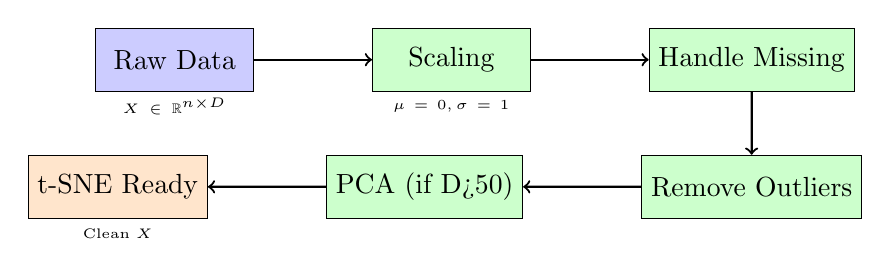
\begin{tikzpicture}[scale=0.85, node distance=1.5cm]
% Pipeline flow
\node[draw, rectangle, fill=blue!20, minimum width=2cm, minimum height=0.8cm] (raw) {Raw Data};
\node[draw, rectangle, fill=green!20, minimum width=2cm, minimum height=0.8cm, right=of raw] (scale) {Scaling};
\node[draw, rectangle, fill=green!20, minimum width=2cm, minimum height=0.8cm, right=of scale] (missing) {Handle Missing};
\node[draw, rectangle, fill=green!20, minimum width=2cm, minimum height=0.8cm, below=0.8cm of missing] (outlier) {Remove Outliers};
\node[draw, rectangle, fill=green!20, minimum width=2cm, minimum height=0.8cm, left=of outlier] (pca) {PCA (if D>50)};
\node[draw, rectangle, fill=orange!20, minimum width=2cm, minimum height=0.8cm, left=of pca] (tsne) {t-SNE Ready};

% Arrows
\draw[->, thick] (raw) -- (scale);
\draw[->, thick] (scale) -- (missing);
\draw[->, thick] (missing) -- (outlier);
\draw[->, thick] (outlier) -- (pca);
\draw[->, thick] (pca) -- (tsne);

% Annotations
\node[font=\tiny, text width=2cm, align=center] at ($(raw)+(0,-0.7)$) {$X \in \mathbb{R}^{n \times D}$};
\node[font=\tiny, text width=2cm, align=center] at ($(scale)+(0,-0.7)$) {$\mu=0, \sigma=1$};
\node[font=\tiny, text width=2cm, align=center] at ($(tsne)+(0,-0.7)$) {Clean $X$};
\end{tikzpicture}
\end{center}

\vspace{0.2cm}
\warning{Bad preprocessing = bad embedding, regardless of parameters!}
\end{frame}

% Slide 40
\begin{frame}{Common Failure Modes and Recovery}
\begin{center}
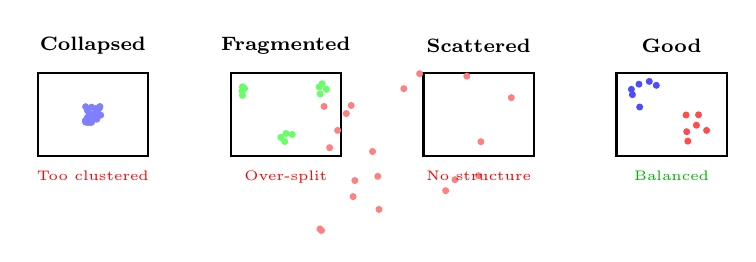
\begin{tikzpicture}[scale=0.7]
% Failure mode 1: Collapsed points
\node at (0,4) {\scriptsize\textbf{Collapsed}};
\draw[thick] (-1,2) rectangle (1,3.5);
\foreach \i in {1,...,25} {
    \pgfmathsetmacro{\x}{rand*0.15}
    \pgfmathsetmacro{\y}{2.75 + rand*0.15}
    \filldraw[blue!50] (\x,\y) circle (1.5pt);
}
\node[below, font=\tiny, text=red] at (0,1.9) {Too clustered};

% Failure mode 2: Fragmented
\node at (3.5,4) {\scriptsize\textbf{Fragmented}};
\draw[thick] (2.5,2) rectangle (4.5,3.5);
\foreach \i in {1,...,4} {
    \pgfmathsetmacro{\x}{2.7 + rand*0.12}
    \pgfmathsetmacro{\y}{3.2 + rand*0.12}
    \filldraw[green!60] (\x,\y) circle (1.5pt);
}
\foreach \i in {1,...,4} {
    \pgfmathsetmacro{\x}{4.2 + rand*0.12}
    \pgfmathsetmacro{\y}{3.2 + rand*0.12}
    \filldraw[green!60] (\x,\y) circle (1.5pt);
}
\foreach \i in {1,...,4} {
    \pgfmathsetmacro{\x}{3.5 + rand*0.12}
    \pgfmathsetmacro{\y}{2.3 + rand*0.12}
    \filldraw[green!60] (\x,\y) circle (1.5pt);
}
\node[below, font=\tiny, text=red] at (3.5,1.9) {Over-split};

% Failure mode 3: Scattered
\node at (7,4) {\scriptsize\textbf{Scattered}};
\draw[thick] (6,2) rectangle (8,3.5);
\foreach \i in {1,...,20} {
    \pgfmathsetmacro{\x}{6 + rand*2}
    \pgfmathsetmacro{\y}{2 + rand*1.5}
    \filldraw[red!50] (\x,\y) circle (1.5pt);
}
\node[below, font=\tiny, text=red] at (7,1.9) {No structure};

% Good result for comparison
\node at (10.5,4) {\scriptsize\textbf{Good}};
\draw[thick] (9.5,2) rectangle (11.5,3.5);
\foreach \i in {1,...,6} {
    \pgfmathsetmacro{\x}{10 + rand*0.25}
    \pgfmathsetmacro{\y}{3.1 + rand*0.25}
    \filldraw[blue!70] (\x,\y) circle (1.5pt);
}
\foreach \i in {1,...,6} {
    \pgfmathsetmacro{\x}{11 + rand*0.25}
    \pgfmathsetmacro{\y}{2.5 + rand*0.25}
    \filldraw[red!70] (\x,\y) circle (1.5pt);
}
\node[below, font=\tiny, text=green!70!black] at (10.5,1.9) {Balanced};
\end{tikzpicture}
\end{center}

\vspace{0.3cm}
\begin{columns}
\column{0.5\textwidth}
\textbf{Collapsed Points:}\\
Increase learning rate\\
Check for duplicates\\
More iterations

\column{0.5\textwidth}
\textbf{Fragmented Clusters:}\\
Increase perplexity\\
Check preprocessing\\
Verify true structure
\end{columns}

\vspace{0.2cm}
\ethics{Failure often reveals data issues, not algorithm issues}
\end{frame}


% Slide 41
\begin{frame}{Real-World Success: Single-Cell Genomics}
\begin{columns}
\column{0.5\textwidth}
\textbf{Challenge:}
\begin{itemize}
\item 10,000+ cells
\item 20,000 genes each
\item Find cell types
\item Identify rare populations
\end{itemize}

\textbf{Pipeline:}
\begin{enumerate}
\item Quality control
\item Normalize counts
\item Select variable genes
\item PCA to 50D
\item t-SNE with perp=30
\item Cluster validation
\end{enumerate}

\column{0.5\textwidth}
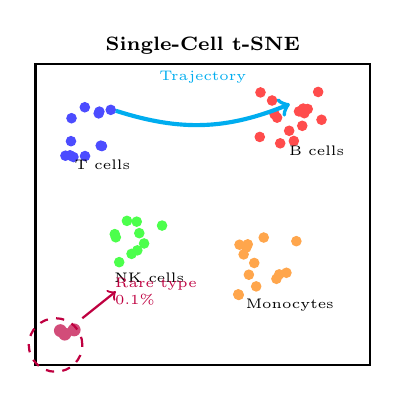
\begin{tikzpicture}[scale=0.85]
% Main embedding space
\draw[thick] (0,0) rectangle (5,4.5);
\node[above] at (2.5,4.5) {\scriptsize\textbf{Single-Cell t-SNE}};

% Major cell type clusters
\foreach \i in {1,...,12} {
    \pgfmathsetmacro{\x}{0.8 + rand*0.4}
    \pgfmathsetmacro{\y}{3.5 + rand*0.4}
    \filldraw[blue!70] (\x,\y) circle (2pt);
}
\node[font=\tiny] at (1,3) {T cells};

\foreach \i in {1,...,15} {
    \pgfmathsetmacro{\x}{3.8 + rand*0.5}
    \pgfmathsetmacro{\y}{3.7 + rand*0.4}
    \filldraw[red!70] (\x,\y) circle (2pt);
}
\node[font=\tiny] at (4.2,3.2) {B cells};

\foreach \i in {1,...,10} {
    \pgfmathsetmacro{\x}{1.5 + rand*0.4}
    \pgfmathsetmacro{\y}{1.8 + rand*0.4}
    \filldraw[green!70] (\x,\y) circle (2pt);
}
\node[font=\tiny] at (1.7,1.3) {NK cells};

\foreach \i in {1,...,14} {
    \pgfmathsetmacro{\x}{3.5 + rand*0.5}
    \pgfmathsetmacro{\y}{1.5 + rand*0.5}
    \filldraw[orange!70] (\x,\y) circle (2pt);
}
\node[font=\tiny] at (3.8,0.9) {Monocytes};

% Rare cell type (highlighted)
\foreach \i in {1,...,3} {
    \pgfmathsetmacro{\x}{0.5 + rand*0.15}
    \pgfmathsetmacro{\y}{0.5 + rand*0.15}
    \filldraw[purple!70] (\x,\y) circle (2.5pt);
}
\draw[purple, thick, dashed] (0.3,0.3) circle (0.4cm);
\draw[->, purple, thick] (0.7,0.7) -- (1.2,1.1);
\node[font=\tiny, text=purple, align=left] at (1.8,1.1) {Rare type\\0.1\%};

% Trajectory arrow
\draw[->, thick, cyan, line width=1.5pt] (1.2,3.8) to[bend right=20] (3.8,3.9);
\node[font=\tiny, text=cyan] at (2.5,4.3) {Trajectory};
\end{tikzpicture}

\vspace{0.2cm}
\textbf{Discoveries:}
\begin{itemize}
\item Found 0.1\% rare cell type
\item Revealed trajectories
\item Published in Nature
\end{itemize}
\end{columns}

\vspace{0.2cm}
\warning{Biological interpretation requires domain expertise!}
\end{frame}

% Slide 42
\begin{frame}{Real-World Success: Word Embeddings}
\begin{center}
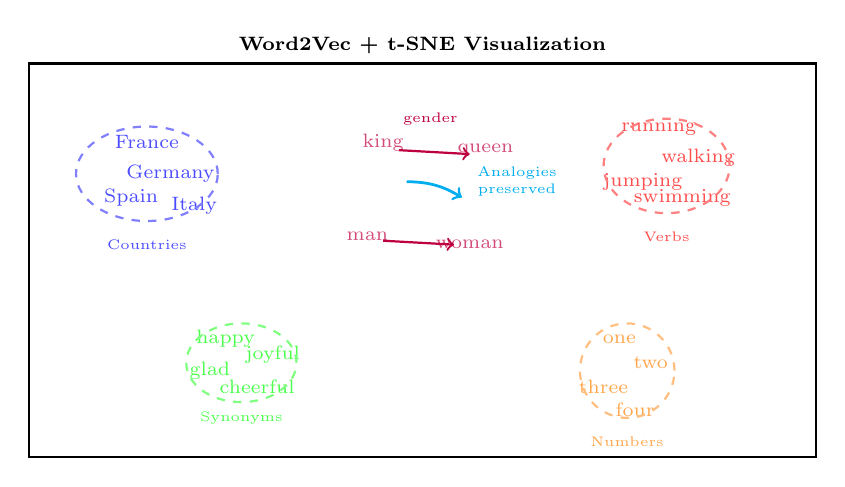
\begin{tikzpicture}[scale=1.0]
% Main embedding space
\draw[thick] (0,0) rectangle (10,5);
\node[above] at (5,5) {\scriptsize\textbf{Word2Vec + t-SNE Visualization}};

% Country cluster
\node[font=\scriptsize, blue!70] at (1.5,4) {France};
\node[font=\scriptsize, blue!70] at (1.8,3.6) {Germany};
\node[font=\scriptsize, blue!70] at (1.3,3.3) {Spain};
\node[font=\scriptsize, blue!70] at (2.1,3.2) {Italy};
\draw[blue!50, dashed, thick] (1.5,3.6) ellipse (0.9cm and 0.6cm);
\node[font=\tiny, blue!70] at (1.5,2.7) {Countries};

% Verb cluster
\node[font=\scriptsize, red!70] at (8,4.2) {running};
\node[font=\scriptsize, red!70] at (8.5,3.8) {walking};
\node[font=\scriptsize, red!70] at (7.8,3.5) {jumping};
\node[font=\scriptsize, red!70] at (8.3,3.3) {swimming};
\draw[red!50, dashed, thick] (8.1,3.7) ellipse (0.8cm and 0.6cm);
\node[font=\tiny, red!70] at (8.1,2.8) {Verbs};

% Royalty/gender analogy
\node[font=\scriptsize, purple!70] at (4.5,4) {king};
\node[font=\scriptsize, purple!70] at (5.8,3.9) {queen};
\node[font=\scriptsize, purple!70] at (4.3,2.8) {man};
\node[font=\scriptsize, purple!70] at (5.6,2.7) {woman};
\draw[->, purple, thick] (4.7,3.9) -- (5.6,3.85);
\draw[->, purple, thick] (4.5,2.75) -- (5.4,2.7);
\node[font=\tiny, purple] at (5.1,4.3) {gender};

% Synonyms cluster
\node[font=\scriptsize, green!70] at (2.5,1.5) {happy};
\node[font=\scriptsize, green!70] at (3.1,1.3) {joyful};
\node[font=\scriptsize, green!70] at (2.3,1.1) {glad};
\node[font=\scriptsize, green!70] at (2.9,0.9) {cheerful};
\draw[green!50, dashed, thick] (2.7,1.2) ellipse (0.7cm and 0.5cm);
\node[font=\tiny, green!70] at (2.7,0.5) {Synonyms};

% Numbers cluster
\node[font=\scriptsize, orange!70] at (7.5,1.5) {one};
\node[font=\scriptsize, orange!70] at (7.9,1.2) {two};
\node[font=\scriptsize, orange!70] at (7.3,0.9) {three};
\node[font=\scriptsize, orange!70] at (7.7,0.6) {four};
\draw[orange!50, dashed, thick] (7.6,1.1) ellipse (0.6cm and 0.6cm);
\node[font=\tiny, orange!70] at (7.6,0.2) {Numbers};

% Analogy annotation
\draw[->, cyan, thick, line width=1pt] (4.8,3.5) to[bend left=15] (5.5,3.3);
\node[font=\tiny, text=cyan, align=center] at (6.2,3.5) {Analogies\\preserved};
\end{tikzpicture}
\end{center}

\vspace{0.2cm}
\begin{columns}
\column{0.5\textwidth}
\textbf{Semantic Clusters:}
\begin{itemize}
\item Countries grouped
\item Verbs together
\item Synonyms clustered
\end{itemize}

\column{0.5\textwidth}
\textbf{Revealed Relationships:}
\begin{itemize}
\item King - Man + Woman $\sim$ Queen
\item Analogies visible
\item Bias detection
\end{itemize}
\end{columns}

\vspace{0.2cm}
\intuition{t-SNE reveals the geometry of language}
\end{frame}

% Slide 43
\begin{frame}{Real-World Success: Deep Learning Features}
\begin{columns}
\column{0.5\textwidth}
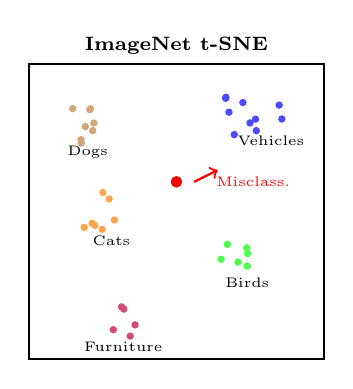
\begin{tikzpicture}[scale=0.75]
% Main embedding space
\draw[thick] (0,0) rectangle (5,5);
\node[above, font=\scriptsize] at (2.5,5) {\textbf{ImageNet t-SNE}};

% Dog breeds cluster
\foreach \i in {1,...,8} {
    \pgfmathsetmacro{\x}{0.8 + rand*0.4}
    \pgfmathsetmacro{\y}{4 + rand*0.4}
    \filldraw[brown!70] (\x,\y) circle (1.5pt);
}
\node[font=\tiny] at (1,3.5) {Dogs};

% Cats cluster
\foreach \i in {1,...,7} {
    \pgfmathsetmacro{\x}{1.2 + rand*0.35}
    \pgfmathsetmacro{\y}{2.5 + rand*0.35}
    \filldraw[orange!70] (\x,\y) circle (1.5pt);
}
\node[font=\tiny] at (1.4,2) {Cats};

% Vehicles cluster
\foreach \i in {1,...,10} {
    \pgfmathsetmacro{\x}{3.8 + rand*0.5}
    \pgfmathsetmacro{\y}{4.2 + rand*0.4}
    \filldraw[blue!70] (\x,\y) circle (1.5pt);
}
\node[font=\tiny] at (4.1,3.7) {Vehicles};

% Birds cluster
\foreach \i in {1,...,6} {
    \pgfmathsetmacro{\x}{3.5 + rand*0.3}
    \pgfmathsetmacro{\y}{1.8 + rand*0.3}
    \filldraw[green!70] (\x,\y) circle (1.5pt);
}
\node[font=\tiny] at (3.7,1.3) {Birds};

% Furniture cluster
\foreach \i in {1,...,5} {
    \pgfmathsetmacro{\x}{1.5 + rand*0.3}
    \pgfmathsetmacro{\y}{0.6 + rand*0.3}
    \filldraw[purple!70] (\x,\y) circle (1.5pt);
}
\node[font=\tiny] at (1.6,0.2) {Furniture};

% Misclassification point
\filldraw[red] (2.5,3) circle (2.5pt);
\draw[->, red, thick] (2.8,3) -- (3.2,3.2);
\node[font=\tiny, text=red] at (3.8,3) {Misclass.};
\end{tikzpicture}

\textbf{ImageNet CNN Features:}
\begin{itemize}
\item ResNet-50 last layer
\item 2048D → 2D
\item 50,000 images
\item 1,000 classes
\end{itemize}

\column{0.5\textwidth}
\textbf{Discoveries:}
\begin{itemize}
\item Hierarchical structure emerges
\item Dogs cluster by breed
\item Vehicles by type
\item Textures group unexpectedly
\item Misclassifications at boundaries
\end{itemize}

\vspace{0.2cm}
\ethics{Visual similarity $\neq$ semantic similarity}
\end{columns}
\end{frame}

% Slide 44
\begin{frame}{Advanced: Parametric t-SNE}
\begin{columns}
\column{0.5\textwidth}
\textbf{Standard t-SNE:}\\
Embeds specific points\\
Cannot handle new data\\
Non-parametric

\vspace{0.3cm}
\textbf{Parametric t-SNE:}\\
Learns function $f_\theta: \mathbb{R}^D \to \mathbb{R}^2$\\
Can embed new points\\
Neural network based

\column{0.5\textwidth}
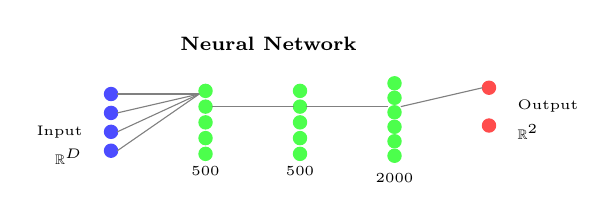
\begin{tikzpicture}[scale=0.8]
% Neural network architecture
\node[font=\scriptsize] at (2.5,5) {\textbf{Neural Network}};

% Input layer
\foreach \i in {1,...,4} {
    \pgfmathsetmacro{\y}{4.5 - \i*0.3}
    \filldraw[blue!70] (0,\y) circle (3pt);
}
\node[left, font=\tiny] at (-0.3,3.6) {Input};
\node[left, font=\tiny] at (-0.3,3.2) {$\mathbb{R}^D$};

% Hidden layer 1
\foreach \i in {1,...,5} {
    \pgfmathsetmacro{\y}{4.5 - \i*0.25}
    \filldraw[green!70] (1.5,\y) circle (3pt);
}
\node[below, font=\tiny] at (1.5,3.2) {500};

% Hidden layer 2
\foreach \i in {1,...,5} {
    \pgfmathsetmacro{\y}{4.5 - \i*0.25}
    \filldraw[green!70] (3,\y) circle (3pt);
}
\node[below, font=\tiny] at (3,3.2) {500};

% Hidden layer 3
\foreach \i in {1,...,6} {
    \pgfmathsetmacro{\y}{4.6 - \i*0.23}
    \filldraw[green!70] (4.5,\y) circle (3pt);
}
\node[below, font=\tiny] at (4.5,3.1) {2000};

% Output layer
\filldraw[red!70] (6,4.3) circle (3pt);
\filldraw[red!70] (6,3.7) circle (3pt);
\node[right, font=\tiny] at (6.3,4) {Output};
\node[right, font=\tiny] at (6.3,3.6) {$\mathbb{R}^2$};

% Connections (sample)
\foreach \i in {1,...,4} {
    \pgfmathsetmacro{\y}{4.5 - \i*0.3}
    \draw[gray, thin] (0.1,\y) -- (1.4,4.2);
}
\draw[gray, thin] (1.6,4) -- (2.9,4);
\draw[gray, thin] (3.1,4) -- (4.4,4);
\draw[gray, thin] (4.6,4) -- (5.9,4.3);
\end{tikzpicture}

\vspace{0.2cm}
\textbf{Architecture:}\\
Input → 500 → 500 → 2000 → 2
\end{columns}

\vspace{0.2cm}
\textbf{Trade-offs:} Lower quality but handles streaming data
\end{frame}

% Slide 45
\begin{frame}{Advanced: Multiscale t-SNE}
\begin{center}
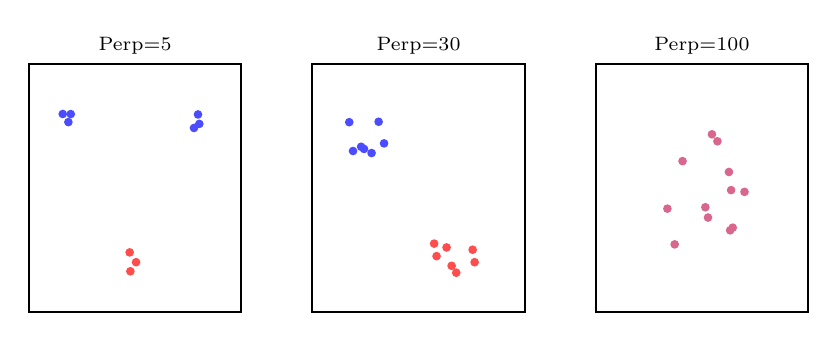
\begin{tikzpicture}[scale=0.9]
% Three different perplexity embeddings
\foreach \perp/\xshift in {5/0, 30/4, 100/8} {
    \begin{scope}[xshift=\xshift cm]
    \draw[thick] (0,0) rectangle (3,3.5);
    \node[above, font=\scriptsize] at (1.5,3.5) {Perp=\perp};
    
    \ifnum\perp=5
        % Very fragmented
        \foreach \i in {1,...,3} {
            \pgfmathsetmacro{\x}{0.5 + rand*0.15}
            \pgfmathsetmacro{\y}{2.7 + rand*0.15}
            \filldraw[blue!70] (\x,\y) circle (1.5pt);
        }
        \foreach \i in {1,...,3} {
            \pgfmathsetmacro{\x}{2.3 + rand*0.15}
            \pgfmathsetmacro{\y}{2.7 + rand*0.15}
            \filldraw[blue!70] (\x,\y) circle (1.5pt);
        }
        \foreach \i in {1,...,3} {
            \pgfmathsetmacro{\x}{1.4 + rand*0.15}
            \pgfmathsetmacro{\y}{0.7 + rand*0.15}
            \filldraw[red!70] (\x,\y) circle (1.5pt);
        }
    \fi
    
    \ifnum\perp=30
        % Balanced
        \foreach \i in {1,...,7} {
            \pgfmathsetmacro{\x}{0.8 + rand*0.3}
            \pgfmathsetmacro{\y}{2.5 + rand*0.3}
            \filldraw[blue!70] (\x,\y) circle (1.5pt);
        }
        \foreach \i in {1,...,7} {
            \pgfmathsetmacro{\x}{2 + rand*0.3}
            \pgfmathsetmacro{\y}{0.8 + rand*0.3}
            \filldraw[red!70] (\x,\y) circle (1.5pt);
        }
    \fi
    
    \ifnum\perp=100
        % More merged
        \foreach \i in {1,...,12} {
            \pgfmathsetmacro{\x}{1.5 + rand*0.6}
            \pgfmathsetmacro{\y}{1.75 + rand*0.8}
            \filldraw[purple!60] (\x,\y) circle (1.5pt);
        }
    \fi
    \end{scope}
}
\end{tikzpicture}
\end{center}

\textbf{Key Idea:} Use multiple perplexities simultaneously
$$p_{ij} = \frac{1}{L}\sum_{l=1}^L p_{ij}^{(l)}$$
where each $p_{ij}^{(l)}$ uses different perplexity

\textbf{Benefits:} Captures structure at all scales\\
\textbf{Cost:} 3× slower computation
\end{frame}

% Slide 46
\begin{frame}{Advanced: Dynamic t-SNE for Time Series}
\begin{columns}
\column{0.5\textwidth}
\textbf{Modified Cost:}
$$C = \sum_t \text{KL}(P^{(t)}||Q^{(t)}) + \lambda\sum_{i,t} \|y_i^{(t)} - y_i^{(t-1)}\|^2$$
First term: Standard t-SNE\\
Second term: Temporal smoothness

\column{0.5\textwidth}
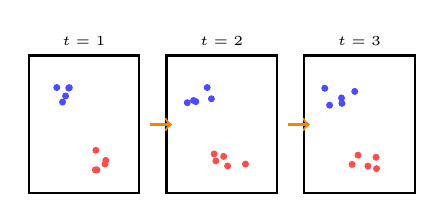
\begin{tikzpicture}[scale=0.7]
% Time series of embeddings
\foreach \t in {1,2,3} {
    \begin{scope}[xshift=\t*2.5 cm]
    \draw[thick] (0,0) rectangle (2,2.5);
    \node[above, font=\tiny] at (1,2.5) {$t=\t$};
    
    % Points evolving over time
    \foreach \i in {1,...,5} {
        \pgfmathsetmacro{\x}{0.5 + rand*0.3 + \t*0.05}
        \pgfmathsetmacro{\y}{1.8 + rand*0.2}
        \filldraw[blue!70] (\x,\y) circle (1.5pt);
    }
    \foreach \i in {1,...,5} {
        \pgfmathsetmacro{\x}{1.2 + rand*0.3 - \t*0.03}
        \pgfmathsetmacro{\y}{0.6 + rand*0.2}
        \filldraw[red!70] (\x,\y) circle (1.5pt);
    }
    
    % Arrows showing temporal connection
    \ifnum\t>1
        \draw[->, orange, thick] (-0.3,1.25) -- (0.1,1.25);
    \fi
    \end{scope}
}
\end{tikzpicture}

\vspace{0.2cm}
\textbf{Applications:}
\begin{itemize}
\item Neural activity
\item Social networks
\item Topic evolution
\item Market dynamics
\end{itemize}
\end{columns}
\end{frame}

% Slide 47
\begin{frame}{Theoretical Foundations: What We Can Prove}
\begin{block}{Guaranteed Properties}
\begin{enumerate}
\item \textbf{Convergence:} Gradient descent reaches local minimum
\item \textbf{Order Preservation:} If $p_{ij} > p_{kl}$ then likely $q_{ij} > q_{kl}$
\item \textbf{Neighborhood Topology:} k-NN graphs approximately preserved
\item \textbf{Information Bound:} KL divergence $\geq$ 0
\end{enumerate}
\end{block}

\begin{block}{NOT Guaranteed}
\begin{enumerate}
\item Global optimum (non-convex problem)
\item Distance preservation (only neighborhoods)
\item Unique solution (depends on initialization)
\item Linear separability preservation
\end{enumerate}
\end{block}

\warning{Despite limitations, empirically very robust!}
\end{frame}

% Slide 48
\begin{frame}{Information Theory Perspective}
\begin{columns}
\column{0.5\textwidth}
\textbf{Information in High-D:}
$$I_{high} = -\sum_{i,j} p_{ij}\log p_{ij}$$
\textbf{Information in Low-D:}
$$I_{low} = -\sum_{i,j} p_{ij}\log q_{ij}$$
\textbf{Information Loss:}
$$\Delta I = \text{KL}(P||Q)$$

\column{0.5\textwidth}
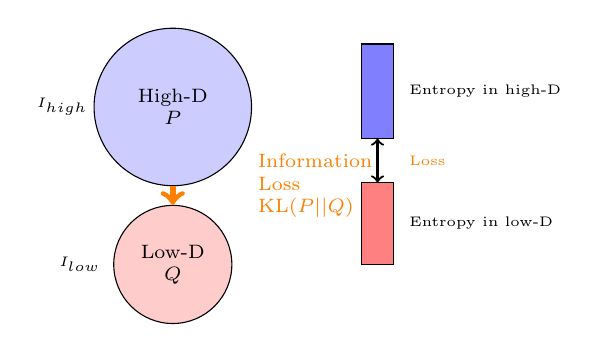
\begin{tikzpicture}[scale=0.8]
% High-D representation
\node[draw, circle, fill=blue!20, minimum size=2cm] (highd) at (0,3) {};
\node[font=\scriptsize, align=center] at (0,3) {High-D\\$P$};
\node[left, font=\tiny] at (-1.2,3) {$I_{high}$};

% Low-D representation
\node[draw, circle, fill=red!20, minimum size=1.5cm] (lowd) at (0,0.5) {};
\node[font=\scriptsize, align=center] at (0,0.5) {Low-D\\$Q$};
\node[left, font=\tiny] at (-1,0.5) {$I_{low}$};

% Information loss arrow
\draw[->, thick, orange, line width=2pt] (highd) -- (lowd);
\node[right, font=\scriptsize, text=orange, align=left] at (1.2,1.75) {Information\\Loss\\$\text{KL}(P||Q)$};

% Entropy bars
\draw[fill=blue!50] (3,2.5) rectangle (3.5,4);
\node[right, font=\tiny] at (3.6,3.25) {Entropy in high-D};

\draw[fill=red!50] (3,0.5) rectangle (3.5,1.8);
\node[right, font=\tiny] at (3.6,1.15) {Entropy in low-D};

\draw[<->, thick] (3.25,1.8) -- (3.25,2.5);
\node[right, font=\tiny, text=orange] at (3.6,2.15) {Loss};
\end{tikzpicture}

\intuition{t-SNE finds the least lossy 2D representation}
\end{columns}
\end{frame}

% Slide 49
\begin{frame}{Physical Analogy: N-Body Simulation}
\begin{center}
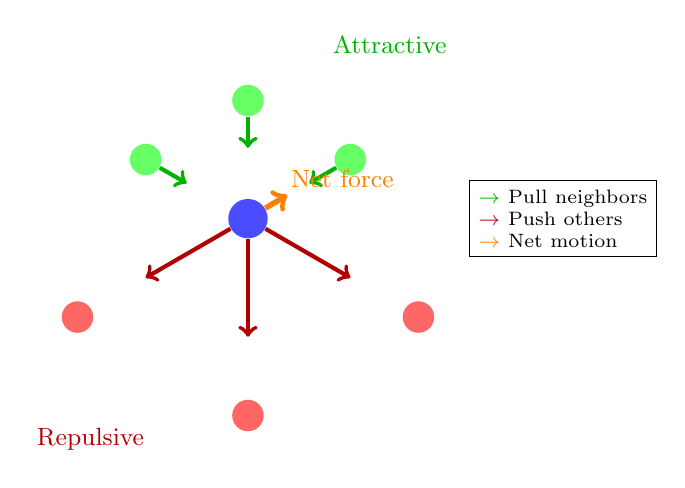
\begin{tikzpicture}[scale=1.0]
% Central point
\node[circle, fill=blue!70, minimum size=0.5cm] (center) at (0,0) {};

% Attractive forces (neighbors)
\foreach \angle in {30, 90, 150} {
    \pgfmathsetmacro{\x}{1.5*cos(\angle)}
    \pgfmathsetmacro{\y}{1.5*sin(\angle)}
    \node[circle, fill=green!60, minimum size=0.4cm] (n\angle) at (\x,\y) {};
    \draw[->, thick, green!70!black, line width=1.5pt] (n\angle) -- ($(center)!0.6!(n\angle)$);
}
\node[font=\small, text=green!70!black] at (1.8,2.2) {Attractive};

% Repulsive forces (distant points)
\foreach \angle in {210, 270, 330} {
    \pgfmathsetmacro{\x}{2.5*cos(\angle)}
    \pgfmathsetmacro{\y}{2.5*sin(\angle)}
    \node[circle, fill=red!60, minimum size=0.4cm] (f\angle) at (\x,\y) {};
    \draw[->, thick, red!70!black, line width=1.5pt] (center) -- ($(f\angle)!0.4!(center)$);
}
\node[font=\small, text=red!70!black] at (-2,-2.8) {Repulsive};

% Force balance annotation
\draw[->, ultra thick, orange, line width=2pt] (center) -- (0.5,0.3);
\node[font=\small, text=orange] at (1.2,0.5) {Net force};

% Legend
\node[font=\scriptsize, align=left, draw, fill=white] at (4,0) {
    \textcolor{green!70!black}{$\rightarrow$} Pull neighbors\\
    \textcolor{red!70!black}{$\rightarrow$} Push others\\
    \textcolor{orange}{$\rightarrow$} Net motion
};
\end{tikzpicture}
\end{center}

\begin{columns}
\column{0.5\textwidth}
\textbf{Attractive Forces:}\\
Pull neighbors together\\
Strength $\propto$ $p_{ij}$\\
Preserve structure

\column{0.5\textwidth}
\textbf{Repulsive Forces:}\\
Push all points apart\\
Create space\\
Prevent collapse
\end{columns}

\vspace{0.2cm}
\colorbox{green!30}{\parbox{0.95\textwidth}{\centering System evolves to mechanical equilibrium = KL minimum}}
\end{frame}

% Slide 50
\begin{frame}{Implementation Options: Choosing Your Tool}
\begin{center}
\begin{tabular}{l|l|l|l}
\textbf{Library} & \textbf{Language} & \textbf{Speed} & \textbf{Best For}\\
\hline
sklearn & Python & Medium & Beginners\\
MulticoreTSNE & Python & Fast & Parallel processing\\
FIt-SNE & C++/Python & Fastest & Large datasets\\
Rtsne & R & Medium & R ecosystem\\
openTSNE & Python & Fast & Research\\
RAPIDS cuML & CUDA & Very Fast & GPU acceleration\\
TensorBoard & Web & Medium & Interactive
\end{tabular}
\end{center}

\vspace{0.3cm}
\textbf{Recommendations:}
\begin{itemize}
\item Start with sklearn for learning
\item Use FIt-SNE or openTSNE for production
\item GPU only worth it for >100K points
\end{itemize}
\end{frame}

% Slide 51
\begin{frame}{Hyperparameter Tuning: Systematic Approach}
\begin{columns}
\column{0.5\textwidth}
\textbf{Grid Search Space:}
\begin{itemize}
\item Perplexity: [5, 10, 20, 30, 50]
\item Learning rate: [10, 100, 200, 500]
\item Iterations: [1000, 2000, 5000]
\item Early exag: [4, 12, 20]
\end{itemize}
Total: 180 combinations

\column{0.5\textwidth}
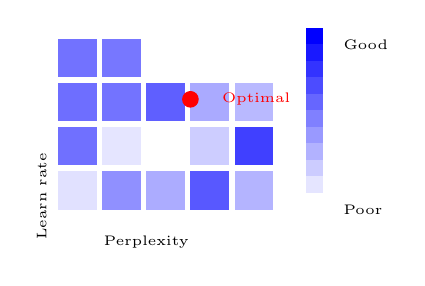
\begin{tikzpicture}[scale=0.7]
% Grid search visualization with proper color clamping
\foreach \x in {0,...,4} {
    \foreach \y in {0,...,3} {
        \pgfmathsetmacro{\randval}{rand}
        \pgfmathsetmacro{\quality}{20 + \randval*60}
        \pgfmathsetmacro{\clampedquality}{min(100, max(0, \quality))}
        \fill[blue!\clampedquality] (\x*0.8,\y*0.8) rectangle ++(0.7,0.7);
    }
}
\node[below, font=\tiny] at (1.6,-0.3) {Perplexity};
\node[left, font=\tiny, rotate=90] at (-0.3,1.2) {Learn rate};

% Optimal point
\filldraw[red] (2.4,2) circle (4pt);
\node[right, font=\tiny, text=red] at (2.8,2) {Optimal};

% Color bar legend
\foreach \i in {0,...,10} {
    \pgfmathsetmacro{\qual}{10*\i}
    \fill[blue!\qual] (4.5,\i*0.3) rectangle (4.8,\i*0.3+0.3);
}
\node[right, font=\tiny] at (5,0) {Poor};
\node[right, font=\tiny] at (5,3) {Good};
\end{tikzpicture}

\vspace{0.2cm}
\textbf{Better: Bayesian Optimization}\\
Reduces search from 180 to ~30
\end{columns}

\vspace{0.2cm}
\warning{Default parameters are rarely optimal!}
\end{frame}

% Slide 52
\begin{frame}{Making t-SNE More Interpretable}
\begin{columns}
\column{0.5\textwidth}
\textbf{Feature Attribution:}

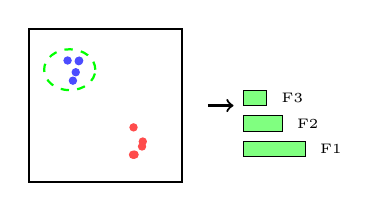
\begin{tikzpicture}[scale=0.65]
% t-SNE embedding
\draw[thick] (0,0) rectangle (3,3);
\foreach \i in {1,...,5} {
    \pgfmathsetmacro{\x}{0.8 + rand*0.3}
    \pgfmathsetmacro{\y}{2.2 + rand*0.3}
    \filldraw[blue!70] (\x,\y) circle (2pt);
}
\foreach \i in {1,...,5} {
    \pgfmathsetmacro{\x}{2 + rand*0.3}
    \pgfmathsetmacro{\y}{0.8 + rand*0.3}
    \filldraw[red!70] (\x,\y) circle (2pt);
}

% Selected cluster
\draw[green, thick, dashed] (0.8,2.2) ellipse (0.5cm and 0.4cm);

% Feature importance bars
\draw[->, thick] (3.5,1.5) -- (4,1.5);
\foreach \i/\val in {1/0.8, 2/0.5, 3/0.3} {
    \draw[fill=green!50] (4.2,\i*0.5) rectangle (4.2+\val*1.5,\i*0.5+0.3);
    \node[right, font=\tiny] at (4.2+\val*1.5+0.1,\i*0.5+0.15) {F\i};
}
\end{tikzpicture}

Which features drive clustering?

\column{0.5\textwidth}
\textbf{Confidence Regions:}

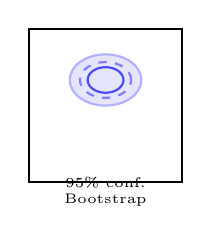
\begin{tikzpicture}[scale=0.65]
% Main embedding
\draw[thick] (0,0) rectangle (3,3);

% Cluster with confidence
\foreach \i in {1,...,6} {
    \pgfmathsetmacro{\x}{1.5 + rand*0.25}
    \pgfmathsetmacro{\y}{2 + rand*0.25}
    \filldraw[blue!70] (\x,\y) circle (2pt);
}

% Confidence ellipses
\draw[blue!30, thick, fill=blue!10] (1.5,2) ellipse (0.7cm and 0.5cm);
\draw[blue!50, thick, dashed] (1.5,2) ellipse (0.5cm and 0.35cm);
\draw[blue!70, thick] (1.5,2) ellipse (0.35cm and 0.25cm);

\node[below, font=\tiny, align=center] at (1.5,0.3) {95\% conf.\\Bootstrap};
\end{tikzpicture}

Bootstrap to show uncertainty
\end{columns}

\vspace{0.3cm}
\textbf{Interactive Explanations:}
\begin{itemize}
\item Click point → show raw features
\item Select region → statistics summary
\item Hover → nearest neighbors in high-D
\end{itemize}
\end{frame}

% Slide 53
\begin{frame}{Troubleshooting: Quick Reference}
\begin{center}
\begin{tabular}{l|l}
\textbf{Problem} & \textbf{Solution}\\
\hline
Points in straight lines & Increase iterations\\
Single ball of points & Increase learning rate\\
Clusters fragmented & Increase perplexity\\
Points scattered randomly & Decrease learning rate\\
NaN in output & Check for duplicate points\\
Very slow convergence & Use PCA preprocessing\\
Different runs very different & Increase iterations\\
Known clusters not separated & Check data scaling\\
Outliers dominate & Remove or downweight\\
Memory error & Use Barnes-Hut
\end{tabular}
\end{center}

\colorbox{yellow!30}{90\% of problems are scaling or perplexity!}
\end{frame}

% Slide 54
\begin{frame}{Future Research Directions}
\begin{block}{Active Areas}
\begin{enumerate}
\item \textbf{Theory:} Convergence guarantees, optimal kernels
\item \textbf{Algorithms:} Linear time exact algorithms
\item \textbf{Extensions:} Graph t-SNE, supervised variants
\item \textbf{Interpretability:} Uncertainty quantification
\end{enumerate}
\end{block}

\textbf{Emerging Alternatives:}
\begin{itemize}
\item PaCMAP (2021): Local + global preservation
\item TriMap (2019): Triplet constraints
\item NCVis (2020): Noise contrastive learning
\end{itemize}

\intuition{t-SNE remains gold standard but field evolving rapidly}
\end{frame}

% Slide 55
\begin{frame}{Ethical Considerations: Responsible Use}
\begin{center}
\colorbox{red!30}{\Large\textbf{With Great Visualization Comes Great Responsibility}}
\end{center}

\textbf{Potential Misuses:}
\begin{enumerate}
\item Creating false patterns from noise
\item Amplifying existing biases
\item Misleading with distances/sizes
\item Cherry-picking favorable runs
\end{enumerate}

\textbf{Best Practices:}
\begin{enumerate}
\item Always validate statistically
\item Report all parameters and preprocessing
\item Show multiple runs/perplexities
\item Include uncertainty measures
\item Document limitations explicitly
\end{enumerate}

\ethics{Your visualization may influence important decisions!}
\end{frame}

% Slide 56
\begin{frame}{Complete Validation Protocol}
\begin{block}{Publication Checklist}
\begin{enumerate}
\item[$\square$] Preprocessing documented
\item[$\square$] Parameters reported (perp, $\eta$, iterations)
\item[$\square$] Multiple runs ($\geq$10)
\item[$\square$] Stability metrics computed
\item[$\square$] NPr(k) reported
\item[$\square$] Trustworthiness measured
\item[$\square$] Perplexity sweep performed
\item[$\square$] Subsample validation done
\item[$\square$] Known structure verified
\item[$\square$] Limitations discussed
\end{enumerate}
\end{block}

\warning{Never publish single t-SNE run without validation!}
\end{frame}

% Slide 57
\begin{frame}{Summary: Key Takeaways}
\begin{enumerate}
\item \textbf{Information > Distance:} t-SNE preserves probability distributions
\item \textbf{Maximum Entropy:} Gaussian kernel emerges naturally
\item \textbf{Heavy Tails:} Student's t solves crowding
\item \textbf{Asymmetric Loss:} Neighbors matter more
\item \textbf{Adaptive Bandwidth:} Perplexity handles density
\item \textbf{Forces:} Gradient is attractive + repulsive forces
\item \textbf{Validation:} Always quantify quality
\item \textbf{Interpretation:} Only trust local structure
\item \textbf{Ethics:} Document and communicate limitations
\item \textbf{Practice:} Multiple runs essential
\end{enumerate}

\colorbox{green!30}{Master these concepts and you master t-SNE!}
\end{frame}

% Slide 58
\begin{frame}{Practical Workflow Checklist}
\begin{columns}
\column{0.5\textwidth}
\textbf{Before t-SNE:}
\begin{itemize}
\item[$\square$] Scale features
\item[$\square$] Handle missing data
\item[$\square$] Remove outliers
\item[$\square$] PCA if D > 50
\item[$\square$] Document everything
\end{itemize}

\textbf{Running t-SNE:}
\begin{itemize}
\item[$\square$] Try perp = 5, 30, 50
\item[$\square$] Ensure convergence
\item[$\square$] Run 5+ times
\item[$\square$] Save seeds
\item[$\square$] Monitor for errors
\end{itemize}

\column{0.5\textwidth}
\textbf{After t-SNE:}
\begin{itemize}
\item[$\square$] Compute NPr
\item[$\square$] Check stability
\item[$\square$] Validate structure
\item[$\square$] Create interactive viz
\item[$\square$] Write methods section
\end{itemize}

\vspace{0.5cm}
\colorbox{yellow!30}{Print and keep handy!}
\end{columns}
\end{frame}

% Slide 59
\begin{frame}{Test Your Understanding}
\textbf{Conceptual Questions:}
\begin{enumerate}
\item Why different distributions in high-D vs low-D?
\item What does perplexity encode?
\item Why is KL divergence asymmetric important?
\end{enumerate}

\textbf{Practical Questions:}
\begin{enumerate}
\setcounter{enumi}{3}
\item Your embedding shows a ball. What's wrong?
\item When use PCA before t-SNE?
\item How validate quality?
\end{enumerate}

\textbf{Advanced Questions:}
\begin{enumerate}
\setcounter{enumi}{6}
\item Derive gradient from cost function
\item Why Barnes-Hut for repulsive forces only?
\item How modify for temporal data?
\end{enumerate}

\colorbox{green!30}{Can you answer all 9? You've mastered t-SNE!}
\end{frame}

% Slide 60
\begin{frame}{Resources for Continued Learning}
\textbf{Essential Papers:}
\begin{itemize}
\item Van der Maaten \& Hinton (2008) - Original t-SNE
\item Kobak \& Berens (2019) - Art of using t-SNE
\item Belkina et al. (2019) - Automated optimization
\end{itemize}

\textbf{Interactive Resources:}
\begin{itemize}
\item Distill.pub - "How to Use t-SNE Effectively"
\item projector.tensorflow.org - Try it yourself
\item github.com/pavlin-policar/openTSNE
\end{itemize}

\textbf{Code Repository:}\\
\texttt{github.com/course/tsne-masterclass}\\
All slides, code, and demos available

\begin{center}
\colorbox{blue!30}{\textbf{Start with Distill.pub - best visual explanation!}}
\end{center}
\end{frame}

% Slide 61
\begin{frame}{Deep Dive: The Mathematics of Information Preservation}
\textbf{Shannon's Information Content:}
$$I(x) = -\log_2 P(x) \text{ bits}$$

\textbf{Applied to Neighborhoods:}
\begin{align}
\text{Surprise of } j \text{ being neighbor: } &-\log p_{j|i}\\
\text{Expected surprise (entropy): } H(P_i) &= -\sum_j p_{j|i}\log p_{j|i}\\
\text{Information lost using } Q_i: \text{KL}(P_i||Q_i) &= \sum_j p_{j|i}\log\frac{p_{j|i}}{q_{j|i}}
\end{align}

\intuition{We're minimizing the "surprise" when using the map instead of true data}

\warning{This is why preserving rare neighbors (high surprise) matters so much!}
\end{frame}

% Slide 62
\begin{frame}{Deep Dive: Why Exactly Student's t with df=1?}
\begin{columns}
\column{0.5\textwidth}
\textbf{General form:}
$$q_{ij} \propto \left(1 + \frac{d_{ij}^2}{\nu}\right)^{-\frac{\nu+1}{2}}$$

where $\nu$ = degrees of freedom

\textbf{Special case $\nu=1$:}
$$q_{ij} \propto (1 + d_{ij}^2)^{-1}$$

\column{0.5\textwidth}
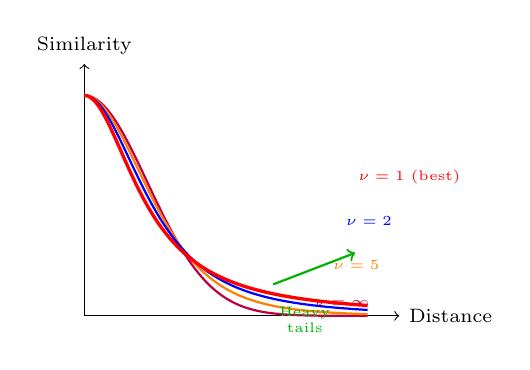
\begin{tikzpicture}[scale=0.8]
% Axes
\draw[->] (0,0) -- (5,0) node[right, font=\scriptsize] {Distance};
\draw[->] (0,0) -- (0,4) node[above, font=\scriptsize] {Similarity};

% Plot different degrees of freedom
% df = infinity (Gaussian)
\draw[purple, thick, domain=0:4.5, samples=100] 
    plot (\x, {3.5*exp(-\x*\x/2)});
\node[right, font=\tiny, text=purple] at (3.5,0.2) {$\nu=\infty$};

% df = 5
\draw[orange, thick, domain=0:4.5, samples=100] 
    plot (\x, {3.5*pow(1+\x*\x/5, -3)});
\node[right, font=\tiny, text=orange] at (3.8,0.8) {$\nu=5$};

% df = 2
\draw[blue, thick, domain=0:4.5, samples=100] 
    plot (\x, {3.5*pow(1+\x*\x/2, -1.5)});
\node[right, font=\tiny, text=blue] at (4,1.5) {$\nu=2$};

% df = 1 (best)
\draw[red, very thick, domain=0:4.5, samples=100] 
    plot (\x, {3.5*pow(1+\x*\x, -1)});
\node[right, font=\tiny, text=red] at (4.2,2.2) {$\nu=1$ (best)};

% Annotation for heavy tails
\draw[->, thick, green!70!black] (3,0.5) -- (4.3,1);
\node[below, font=\tiny, text=green!70!black, align=center] at (3.5,0.3) {Heavy\\tails};
\end{tikzpicture}

\vspace{0.2cm}
\begin{tabular}{l|l}
df & Tail behavior\\
\hline
1 & Heaviest (best)\\
2 & Moderate\\
5 & Light\\
$\infty$ & Gaussian (fails)
\end{tabular}
\end{columns}

\vspace{0.2cm}
\textbf{Mathematical Justification:} df = embedding dimension works optimally\\
For 2D visualization: df = 1 is theoretically optimal!
\end{frame}

% Slide 63
\begin{frame}{Case Study: Debugging a Failed Embedding}
\begin{columns}
\column{0.5\textwidth}
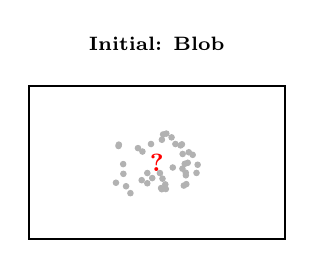
\begin{tikzpicture}[scale=0.65]
% Failed embedding - blob
\node[above] at (2.5,3.5) {\scriptsize\textbf{Initial: Blob}};
\draw[thick] (0,0) rectangle (5,3);
\foreach \i in {1,...,40} {
    \pgfmathsetmacro{\x}{2.5 + rand*0.8}
    \pgfmathsetmacro{\y}{1.5 + rand*0.6}
    \filldraw[gray!60] (\x,\y) circle (1.5pt);
}
\node[text=red, font=\small] at (2.5,1.5) {\textbf{?}};
\end{tikzpicture}

\textbf{Debugging Steps:}
\begin{enumerate}
\item Check data scaling ✗
\item Verify no NaN ✓
\item Increase iterations ✗
\item Adjust learning rate ✗
\item Check duplicates ✓✓✓
\end{enumerate}

\column{0.5\textwidth}
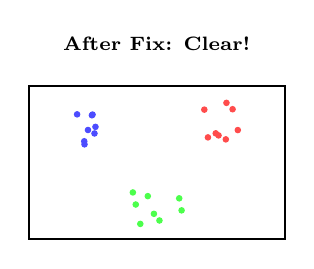
\begin{tikzpicture}[scale=0.65]
% Fixed embedding - clear clusters
\node[above] at (2.5,3.5) {\scriptsize\textbf{After Fix: Clear!}};
\draw[thick] (0,0) rectangle (5,3);
\foreach \i in {1,...,8} {
    \pgfmathsetmacro{\x}{1 + rand*0.4}
    \pgfmathsetmacro{\y}{2.2 + rand*0.4}
    \filldraw[blue!70] (\x,\y) circle (1.5pt);
}
\foreach \i in {1,...,8} {
    \pgfmathsetmacro{\x}{3.8 + rand*0.4}
    \pgfmathsetmacro{\y}{2.3 + rand*0.4}
    \filldraw[red!70] (\x,\y) circle (1.5pt);
}
\foreach \i in {1,...,8} {
    \pgfmathsetmacro{\x}{2.5 + rand*0.5}
    \pgfmathsetmacro{\y}{0.7 + rand*0.4}
    \filldraw[green!70] (\x,\y) circle (1.5pt);
}
\end{tikzpicture}

\textbf{After Removing Duplicates:}\\
Clear structure emerges!

\textbf{Lesson:} 5\% duplicate points destroyed entire embedding
\end{columns}

\vspace{0.2cm}
\ethics{Always check data quality before blaming the algorithm}
\end{frame}

% Slide 64
\begin{frame}{Case Study: Discovering Fraud Patterns}
\begin{columns}
\column{0.5\textwidth}
\textbf{Financial Transaction Data:}
\begin{itemize}
\item 1M transactions
\item 50 features
\item 0.1\% fraud rate
\item Highly imbalanced
\end{itemize}

\textbf{Challenges:}
\begin{itemize}
\item Rare events
\item Mixed data types
\item Temporal patterns
\item High stakes
\end{itemize}

\column{0.5\textwidth}
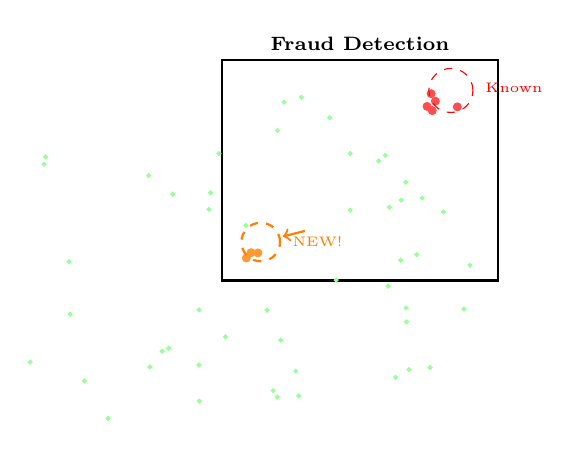
\begin{tikzpicture}[scale=0.7]
\draw[thick] (0,0) rectangle (5,4);
\node[above] at (2.5,4) {\scriptsize\textbf{Fraud Detection}};

% Normal transactions (many)
\foreach \i in {1,...,50} {
    \pgfmathsetmacro{\x}{0.5 + rand*4}
    \pgfmathsetmacro{\y}{0.5 + rand*3}
    \filldraw[green!40] (\x,\y) circle (1pt);
}

% Known fraud cluster
\foreach \i in {1,...,5} {
    \pgfmathsetmacro{\x}{4 + rand*0.3}
    \pgfmathsetmacro{\y}{3.3 + rand*0.3}
    \filldraw[red!70] (\x,\y) circle (2pt);
}
\draw[red, dashed] (4.15,3.45) circle (0.4cm);
\node[right, font=\tiny, text=red] at (4.6,3.5) {Known};

% NEW fraud cluster discovered
\foreach \i in {1,...,3} {
    \pgfmathsetmacro{\x}{0.6 + rand*0.2}
    \pgfmathsetmacro{\y}{0.6 + rand*0.2}
    \filldraw[orange!80] (\x,\y) circle (2pt);
}
\draw[orange, thick, dashed] (0.7,0.7) circle (0.35cm);
\node[right, font=\tiny, text=orange] at (1.1,0.7) {NEW!};
\draw[->, orange, thick] (1.5,0.9) -- (1.1,0.8);
\end{tikzpicture}

\textbf{Discoveries:}
\begin{itemize}
\item New fraud cluster found
\item Saved \$2M in first month
\item Previously unknown pattern
\end{itemize}
\end{columns}

\vspace{0.2cm}
\warning{Always combine with other validation methods for high-stakes decisions}
\end{frame}

% Slide 65
\begin{frame}{Advanced Optimization: Modern Acceleration Techniques}
\begin{columns}
\column{0.5\textwidth}
\textbf{FFT Acceleration (FIt-SNE):}
\begin{itemize}
\item Interpolate on grid
\item Use FFT for forces
\item $O(n)$ complexity
\item 10-50× speedup
\end{itemize}

\textbf{Random Projection Trees:}
\begin{itemize}
\item Multiple trees
\item Average results
\item Better accuracy
\item Moderate speedup
\end{itemize}

\column{0.5\textwidth}
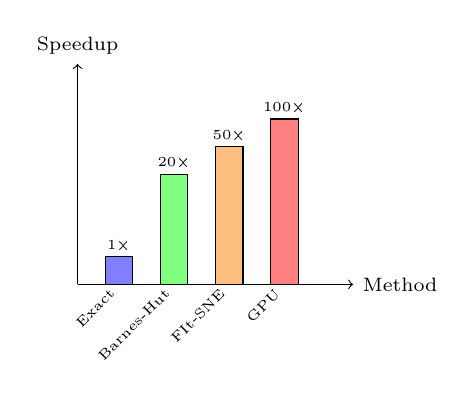
\begin{tikzpicture}[scale=0.7]
% Bar chart comparing methods
\draw[->] (0,0) -- (0,4) node[above, font=\scriptsize] {Speedup};
\draw[->] (0,0) -- (5,0) node[right, font=\scriptsize] {Method};

% Bars
\draw[fill=blue!50] (0.5,0) rectangle (1,0.5);
\node[below, font=\tiny, rotate=45, anchor=east] at (0.75,0) {Exact};

\draw[fill=green!50] (1.5,0) rectangle (2,2);
\node[below, font=\tiny, rotate=45, anchor=east] at (1.75,0) {Barnes-Hut};

\draw[fill=orange!50] (2.5,0) rectangle (3,2.5);
\node[below, font=\tiny, rotate=45, anchor=east] at (2.75,0) {FIt-SNE};

\draw[fill=red!50] (3.5,0) rectangle (4,3);
\node[below, font=\tiny, rotate=45, anchor=east] at (3.75,0) {GPU};

% Values
\node[font=\tiny] at (0.75,0.7) {1×};
\node[font=\tiny] at (1.75,2.2) {20×};
\node[font=\tiny] at (2.75,2.7) {50×};
\node[font=\tiny] at (3.75,3.2) {100×};
\end{tikzpicture}

\vspace{0.2cm}
\begin{tabular}{l|r|r}
Method & Time & Quality\\
\hline
Exact & 100\% & 100\%\\
Barnes-Hut & 5\% & 98\%\\
FIt-SNE & 2\% & 99\%\\
GPU & 1\% & 98\%
\end{tabular}
\end{columns}
\end{frame}

% Slide 66
\begin{frame}{Handling Streaming Data: Online t-SNE}
\begin{center}
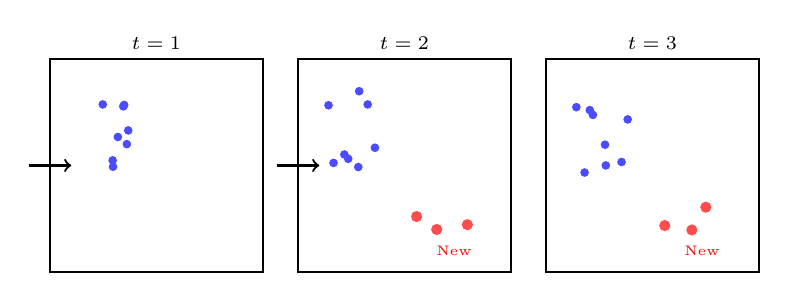
\begin{tikzpicture}[scale=0.9]
% Three time steps
\foreach \t in {1,2,3} {
    \begin{scope}[xshift=\t*3.5 cm]
    \draw[thick] (0,0) rectangle (3,3);
    \node[above, font=\scriptsize] at (1.5,3) {$t=\t$};
    
    % Existing points
    \foreach \i in {1,...,8} {
        \pgfmathsetmacro{\x}{0.8 + rand*0.4}
        \pgfmathsetmacro{\y}{2 + rand*0.6}
        \filldraw[blue!70] (\x,\y) circle (1.5pt);
    }
    
    % New incoming points
    \ifnum\t>1
        \foreach \i in {1,...,3} {
            \pgfmathsetmacro{\x}{2 + rand*0.4}
            \pgfmathsetmacro{\y}{0.8 + rand*0.4}
            \filldraw[red!70] (\x,\y) circle (2pt);
        }
        \node[font=\tiny, text=red] at (2.2,0.3) {New};
    \fi
    \end{scope}
}

% Arrows showing time flow
\draw[->, thick] (3.2,1.5) -- (3.8,1.5);
\draw[->, thick] (6.7,1.5) -- (7.3,1.5);
\end{tikzpicture}
\end{center}

\textbf{Three Approaches:}
\begin{enumerate}
\item \textbf{Periodic Recomputation:} Best quality, positions change
\item \textbf{Parametric Extension:} Fast, lower quality, drift
\item \textbf{Incremental:} Balance, complex implementation
\end{enumerate}

\intuition{No perfect solution - choose based on stability vs quality needs}
\end{frame}

% Slide 67
\begin{frame}{Cross-Validation for t-SNE}
\begin{columns}
\column{0.5\textwidth}
\textbf{Validation Protocol:}
\begin{enumerate}
\item Split data 80/20
\item Embed training set
\item Project test set
\item Compare structures
\item Repeat 5-fold
\end{enumerate}

\textbf{Quality Metrics:}
\begin{itemize}
\item Procrustes distance
\item Neighborhood overlap
\item Cluster consistency
\end{itemize}

\column{0.5\textwidth}
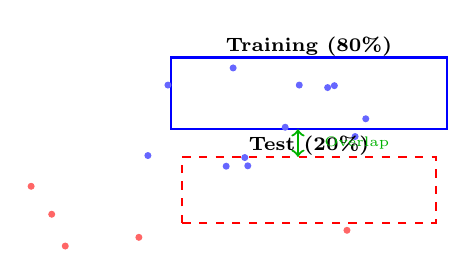
\begin{tikzpicture}[scale=0.7]
% Training embedding
\node[font=\scriptsize] at (2.5,5) {\textbf{Training (80\%)}};
\draw[thick, blue] (0,3.5) rectangle (5,4.8);
\foreach \i in {1,...,12} {
    \pgfmathsetmacro{\x}{0.5 + rand*4}
    \pgfmathsetmacro{\y}{3.7 + rand*1}
    \filldraw[blue!60] (\x,\y) circle (1.5pt);
}

% Test embedding (overlaid)
\node[font=\scriptsize] at (2.5,3.2) {\textbf{Test (20\%)}};
\draw[thick, red, dashed] (0.2,1.8) rectangle (4.8,3);
\foreach \i in {1,...,5} {
    \pgfmathsetmacro{\x}{0.7 + rand*3.5}
    \pgfmathsetmacro{\y}{2 + rand*0.8}
    \filldraw[red!60] (\x,\y) circle (1.5pt);
}

% Overlap indicator
\draw[<->, green!70!black, thick] (2.3,3) -- (2.3,3.5);
\node[right, font=\tiny, text=green!70!black] at (2.6,3.25) {Overlap};
\end{tikzpicture}

\textbf{Interpretation:}
\begin{itemize}
\item High overlap = stable
\item Low overlap = overfitting
\item Adjust perplexity accordingly
\end{itemize}
\end{columns}
\end{frame}

% Slide 68
\begin{frame}{Combining with Other Methods: Ensemble Approaches}
\begin{center}
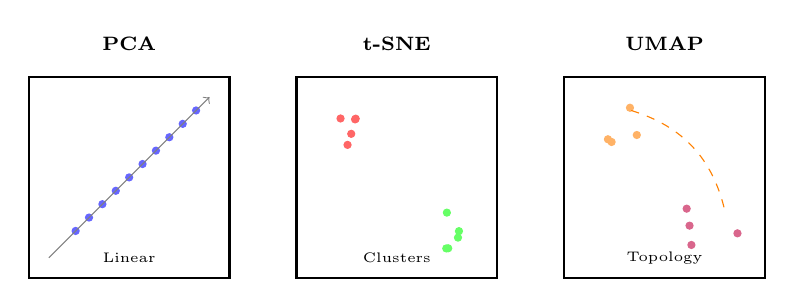
\begin{tikzpicture}[scale=0.85]
% Three different method results
% PCA
\begin{scope}
\node[font=\scriptsize] at (1.5,3.5) {\textbf{PCA}};
\draw[thick] (0,0) rectangle (3,3);
\foreach \i in {1,...,10} {
    \pgfmathsetmacro{\x}{0.5 + \i*0.2}
    \pgfmathsetmacro{\y}{0.5 + \i*0.2}
    \filldraw[blue!60] (\x,\y) circle (1.5pt);
}
\draw[->, gray] (0.3,0.3) -- (2.7,2.7);
\node[font=\tiny] at (1.5,0.3) {Linear};
\end{scope}

% t-SNE
\begin{scope}[xshift=4cm]
\node[font=\scriptsize] at (1.5,3.5) {\textbf{t-SNE}};
\draw[thick] (0,0) rectangle (3,3);
\foreach \i in {1,...,5} {
    \pgfmathsetmacro{\x}{0.7 + rand*0.3}
    \pgfmathsetmacro{\y}{2.2 + rand*0.3}
    \filldraw[red!60] (\x,\y) circle (1.5pt);
}
\foreach \i in {1,...,5} {
    \pgfmathsetmacro{\x}{2.2 + rand*0.3}
    \pgfmathsetmacro{\y}{0.7 + rand*0.3}
    \filldraw[green!60] (\x,\y) circle (1.5pt);
}
\node[font=\tiny] at (1.5,0.3) {Clusters};
\end{scope}

% UMAP
\begin{scope}[xshift=8cm]
\node[font=\scriptsize] at (1.5,3.5) {\textbf{UMAP}};
\draw[thick] (0,0) rectangle (3,3);
\foreach \i in {1,...,4} {
    \pgfmathsetmacro{\x}{0.8 + rand*0.4}
    \pgfmathsetmacro{\y}{2.3 + rand*0.4}
    \filldraw[orange!60] (\x,\y) circle (1.5pt);
}
\foreach \i in {1,...,4} {
    \pgfmathsetmacro{\x}{2.2 + rand*0.4}
    \pgfmathsetmacro{\y}{0.8 + rand*0.4}
    \filldraw[purple!60] (\x,\y) circle (1.5pt);
}
\draw[orange, dashed] (1,2.5) to[bend left] (2.4,1);
\node[font=\tiny] at (1.5,0.3) {Topology};
\end{scope}
\end{tikzpicture}
\end{center}

\textbf{Complementary Strengths:}
\begin{columns}
\column{0.33\textwidth}
\textbf{PCA}\\
Global structure\\
Linear patterns\\
Fast

\column{0.33\textwidth}
\textbf{t-SNE}\\
Local structure\\
Clusters\\
Non-linear

\column{0.33\textwidth}
\textbf{UMAP}\\
Multi-scale\\
Topology\\
Scalable
\end{columns}

\vspace{0.2cm}
\colorbox{green!30}{\parbox{0.9\textwidth}{\centering Truth emerges from agreement across methods}}
\end{frame}

% Slide 69
\begin{frame}{Critical Analysis: When NOT to Use t-SNE}
\begin{block}{Inappropriate Use Cases}
\begin{enumerate}
\item \textbf{Proving cluster existence:} t-SNE can create false clusters
\item \textbf{Measuring distances:} Only topology preserved
\item \textbf{Real-time analysis:} Too slow for streaming
\item \textbf{Very high-D (>10,000):} Computational limits
\item \textbf{Precise reproduction:} Stochastic nature
\end{enumerate}
\end{block}

\textbf{Better Alternatives:}
\begin{itemize}
\item Hypothesis testing → Statistical tests
\item Distance preservation → MDS
\item Speed critical → UMAP or PCA
\item Reproducibility → Deterministic methods
\end{itemize}

\vspace{0.2cm}
\ethics{Using wrong tool can lead to wrong conclusions}
\end{frame}

% Slide 70
\begin{frame}{Memory Optimization Strategies}
\begin{columns}
\column{0.5\textwidth}
\textbf{Memory Requirements:}
\begin{tabular}{l|r}
Component & Memory\\
\hline
Distance matrix & $O(n^2)$\\
P matrix (dense) & $O(n^2)$\\
P matrix (sparse) & $O(nk)$\\
Embeddings & $O(n)$\\
Gradients & $O(n)$
\end{tabular}

\vspace{0.3cm}
\textbf{For 100K points:}\\
Dense: 80GB\\
Sparse: 800MB

\column{0.5\textwidth}
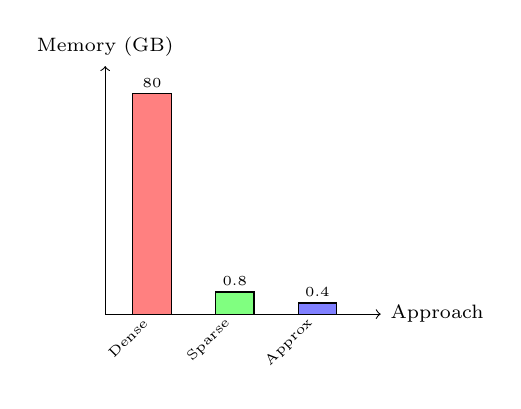
\begin{tikzpicture}[scale=0.7]
% Memory comparison bar chart
\draw[->] (0,0) -- (0,4.5) node[above, font=\scriptsize] {Memory (GB)};
\draw[->] (0,0) -- (5,0) node[right, font=\scriptsize] {Approach};

% Dense
\draw[fill=red!50] (0.5,0) rectangle (1.2,4);
\node[below, font=\tiny, rotate=45, anchor=east] at (0.85,0) {Dense};
\node[font=\tiny] at (0.85,4.2) {80};

% Sparse
\draw[fill=green!50] (2,0) rectangle (2.7,0.4);
\node[below, font=\tiny, rotate=45, anchor=east] at (2.35,0) {Sparse};
\node[font=\tiny] at (2.35,0.6) {0.8};

% Approximate
\draw[fill=blue!50] (3.5,0) rectangle (4.2,0.2);
\node[below, font=\tiny, rotate=45, anchor=east] at (3.85,0) {Approx};
\node[font=\tiny] at (3.85,0.4) {0.4};
\end{tikzpicture}

\textbf{Optimization Tricks:}
\begin{enumerate}
\item Use float32 not float64
\item Sparse P (only k-NN)
\item Chunk distance computation
\item Memory-mapped arrays
\item Approximate methods
\end{enumerate}
\end{columns}
\end{frame}

% Slide 71
\begin{frame}{Publication Standards: Reporting Template}
\begin{block}{Methods Section Template}
"We applied t-SNE (van der Maaten \& Hinton, 2008) using the following protocol:

\textbf{Preprocessing:} Data were scaled to zero mean and unit variance. Missing values were imputed using [method]. PCA was applied to reduce dimensionality from [D] to [d] dimensions, retaining [X]\% of variance.

\textbf{Parameters:} Perplexity = [value], learning rate = [value], iterations = [value], early exaggeration = [value] for [n] iterations.

\textbf{Validation:} The embedding was computed [N] times with different random seeds. Mean pairwise correlation = [value] ± [std]. Neighborhood preservation (k=[perp]) = [value].

\textbf{Implementation:} [Package name and version]"
\end{block}

\warning{Incomplete reporting makes work irreproducible}
\end{frame}

% Slide 72
\begin{frame}{Common Misinterpretations in Literature}
\begin{columns}
\column{0.5\textwidth}
\textbf{Real Examples (Anonymized):}
\begin{enumerate}
\item "Distance between clusters shows evolutionary relationship"
\item "Larger clusters contain more samples"
\item "Position indicates importance"
\item "Single run proves structure"
\end{enumerate}

\column{0.5\textwidth}
\textbf{Corrections:}
\begin{enumerate}
\item Inter-cluster distance meaningless
\item Visual size $\neq$ sample count
\item Position is arbitrary
\item Multiple runs essential
\end{enumerate}
\end{columns}

\vspace{0.3cm}
\colorbox{red!30}{\parbox{0.9\textwidth}{\centering\textbf{These errors led to paper retractions!}}}

\vspace{0.2cm}
\ethics{Peer reviewers should check t-SNE usage carefully}
\end{frame}

% Slide 73
\begin{frame}{Interactive Demo: Building Intuition}
\begin{center}
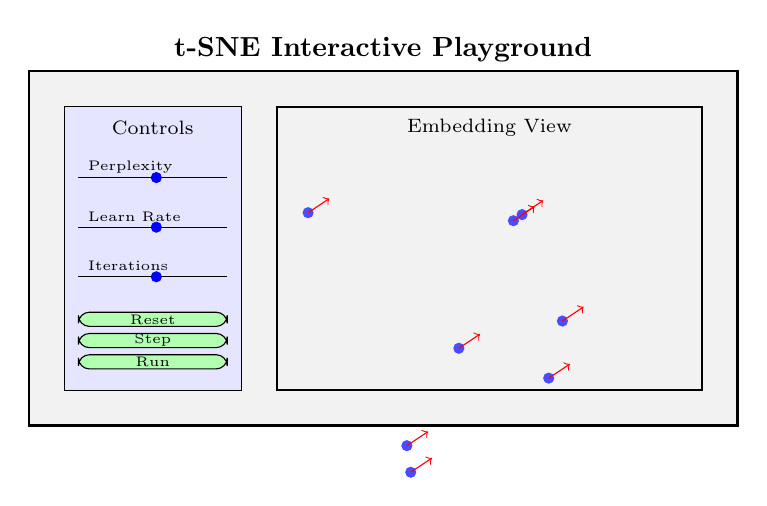
\begin{tikzpicture}[scale=0.9]
% Interactive playground mockup
\draw[thick, fill=gray!10] (0,0) rectangle (10,5);
\node[above] at (5,5) {\textbf{t-SNE Interactive Playground}};

% Control panel
\draw[fill=blue!10] (0.5,0.5) rectangle (3,4.5);
\node[font=\scriptsize] at (1.75,4.2) {Controls};

% Sliders
\foreach \y/\label in {3.5/Perplexity, 2.8/Learn Rate, 2.1/Iterations} {
    \draw (0.7,\y) -- (2.8,\y);
    \filldraw[blue] (1.8,\y) circle (2pt);
    \node[right, font=\tiny] at (0.7,\y+0.15) {\label};
}

% Buttons
\foreach \y/\label in {1.5/Reset, 1.2/Step, 0.9/Run} {
    \draw[fill=green!30, rounded corners] (0.7,\y-0.1) rectangle (2.8,\y+0.1);
    \node[font=\tiny] at (1.75,\y) {\label};
}

% Visualization area
\draw[thick] (3.5,0.5) rectangle (9.5,4.5);
\node[font=\scriptsize] at (6.5,4.2) {Embedding View};

% Sample points with force vectors
\foreach \i in {1,...,8} {
    \pgfmathsetmacro{\x}{4.5 + rand*4}
    \pgfmathsetmacro{\y}{1.5 + rand*2.5}
    \filldraw[blue!70] (\x,\y) circle (2pt);
    \draw[->, red, thin] (\x,\y) -- (\x+0.3,\y+0.2);
}
\end{tikzpicture}
\end{center}

\textbf{Interactive Playground Features:}
\begin{itemize}
\item Drag points in high-D, see low-D update
\item Adjust perplexity in real-time
\item Visualize force vectors
\item Show optimization path
\item Compare different kernels
\end{itemize}

\textit{Access at: tsne-playground.github.io}

\intuition{Playing with the algorithm builds deeper understanding than equations alone}
\end{frame}

% Slide 74
\begin{frame}{Performance Benchmarks: Real-World Datasets}
\begin{center}
\begin{tabular}{l|r|r|r|r}
\textbf{Dataset} & \textbf{Points} & \textbf{Dims} & \textbf{Time} & \textbf{Quality}\\
\hline
MNIST & 70K & 784 & 45 min & 0.92\\
CIFAR-10 & 60K & 3072 & 38 min & 0.88\\
20 Newsgroups & 18K & 10000 & 15 min & 0.85\\
Single-cell & 30K & 20000 & 25 min & 0.90\\
Word2Vec & 10K & 300 & 8 min & 0.94\\
Financial & 100K & 50 & 55 min & 0.87
\end{tabular}
\end{center}

\textbf{Setup:} Intel i7, 32GB RAM, openTSNE, perplexity=30\\
\textbf{Quality:} Neighborhood preservation at k=30

\vspace{0.3cm}
\warning{Your results will vary based on hardware and implementation}
\end{frame}

% Slide 75
\begin{frame}{The Art of Perplexity Selection}
\begin{center}
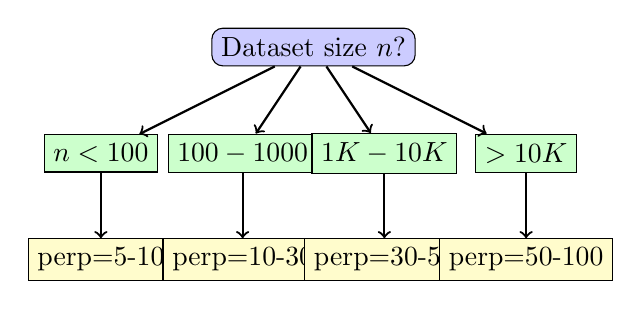
\begin{tikzpicture}[scale=0.9]
% Decision tree for perplexity
\node[draw, fill=blue!20, rounded corners] (start) at (0,4) {Dataset size $n$?};

\node[draw, fill=green!20] (small) at (-3,2.5) {$n < 100$};
\node[draw, fill=green!20] (medium) at (-1,2.5) {$100-1000$};
\node[draw, fill=green!20] (large) at (1,2.5) {$1K-10K$};
\node[draw, fill=green!20] (huge) at (3,2.5) {$>10K$};

\node[draw, fill=yellow!20] (p1) at (-3,1) {perp=5-10};
\node[draw, fill=yellow!20] (p2) at (-1,1) {perp=10-30};
\node[draw, fill=yellow!20] (p3) at (1,1) {perp=30-50};
\node[draw, fill=yellow!20] (p4) at (3,1) {perp=50-100};

\draw[->, thick] (start) -- (small);
\draw[->, thick] (start) -- (medium);
\draw[->, thick] (start) -- (large);
\draw[->, thick] (start) -- (huge);

\draw[->, thick] (small) -- (p1);
\draw[->, thick] (medium) -- (p2);
\draw[->, thick] (large) -- (p3);
\draw[->, thick] (huge) -- (p4);
\end{tikzpicture}
\end{center}

\textbf{Data-Driven Guidelines:}
\begin{columns}
\column{0.5\textwidth}
\begin{itemize}
\item Dense manifolds: 50-100
\item Clear clusters: 20-50
\item Sparse data: 5-20
\item Mixed density: 30 (default)
\end{itemize}

\column{0.5\textwidth}
\begin{itemize}
\item $n < 100$: perp = 5-10
\item $n = 100-1000$: perp = 10-30
\item $n = 1000-10000$: perp = 30-50
\item $n > 10000$: perp = 50-100
\end{itemize}
\end{columns}

\vspace{0.2cm}
\colorbox{green!30}{\parbox{0.9\textwidth}{\centering Always try multiple values and look for consistency}}
\end{frame}

% Slide 76
\begin{frame}{Integration with Machine Learning Pipelines}
\begin{center}
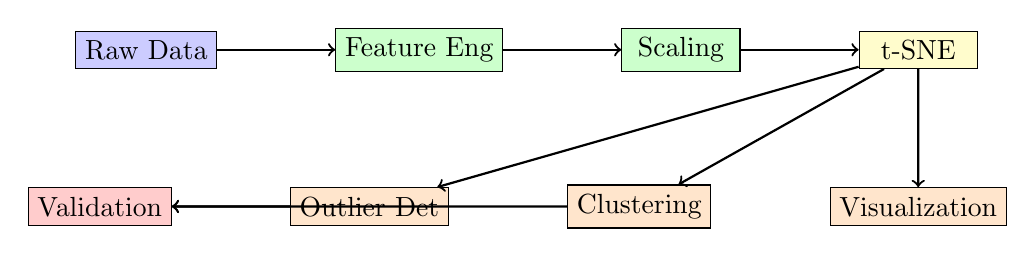
\begin{tikzpicture}[scale=0.85, node distance=1.5cm]
% Top row - preprocessing
\node[draw, fill=blue!20, minimum width=1.5cm] (data) {Raw Data};
\node[draw, fill=green!20, minimum width=1.5cm, right=of data] (feat) {Feature Eng};
\node[draw, fill=green!20, minimum width=1.5cm, right=of feat] (scale) {Scaling};
\node[draw, fill=yellow!20, minimum width=1.5cm, right=of scale] (tsne) {t-SNE};

% Bottom row - analysis
\node[draw, fill=orange!20, minimum width=1.5cm, below=of tsne] (viz) {Visualization};
\node[draw, fill=orange!20, minimum width=1.5cm, left=of viz] (cluster) {Clustering};
\node[draw, fill=orange!20, minimum width=1.5cm, left=of cluster] (outlier) {Outlier Det};
\node[draw, fill=red!20, minimum width=1.5cm, left=of outlier] (validate) {Validation};

% Arrows
\draw[->, thick] (data) -- (feat);
\draw[->, thick] (feat) -- (scale);
\draw[->, thick] (scale) -- (tsne);
\draw[->, thick] (tsne) -- (viz);
\draw[->, thick] (tsne) -- (cluster);
\draw[->, thick] (tsne) -- (outlier);
\draw[->, thick] (cluster) -- (validate);
\draw[->, thick] (outlier) -- (validate);
\end{tikzpicture}
\end{center}

\textbf{Best Practices:}
\begin{itemize}
\item t-SNE for exploration, not production
\item Always validate discovered patterns
\item Combine with domain knowledge
\item Document full pipeline
\end{itemize}
\end{frame}

% Slide 77
\begin{frame}{Final Exam: Test Your Mastery}
\textbf{You have this failed t-SNE result:}
\begin{center}
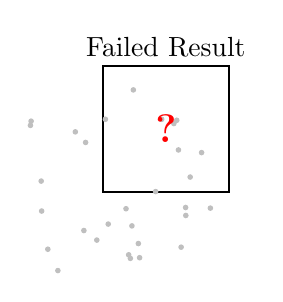
\begin{tikzpicture}[scale=0.4]
\draw[thick] (0,0) rectangle (4,4);
\node[above] at (2,4) {Failed Result};
% Scattered mess
\foreach \i in {1,...,30} {
    \pgfmathsetmacro{\x}{0.5 + rand*3}
    \pgfmathsetmacro{\y}{0.5 + rand*3}
    \filldraw[gray!50] (\x,\y) circle (2pt);
}
\node[text=red, font=\Large] at (2,2) {\textbf{?}};
\end{tikzpicture}
\end{center}

\textbf{Questions:}
\begin{enumerate}
\item List 3 possible causes
\item What diagnostics would you run?
\item Propose fixing sequence
\item How validate the solution?
\end{enumerate}

\pause
\textbf{Expert Answers:}
\small
1. Low learning rate, few iterations, wrong perplexity\\
2. Check convergence, run stability test, sweep perplexity\\
3. Increase $\eta$ → more iterations → adjust perplexity\\
4. NPr metric, multiple runs, known structure test
\end{frame}

% Slide 78
\begin{frame}{The Complete Journey: From Theory to Practice}
\begin{center}
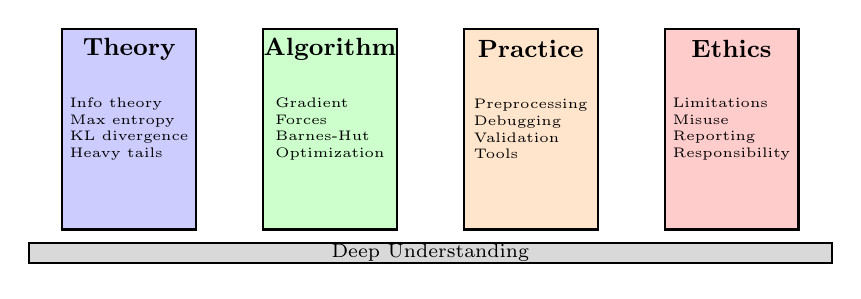
\begin{tikzpicture}[scale=0.85]
% Four pillars
\foreach \x/\label/\color in {0/Theory/blue, 3/Algorithm/green, 6/Practice/orange, 9/Ethics/red} {
    \draw[thick, fill=\color!20] (\x,0) rectangle (\x+2,3);
    \node[font=\small\bfseries] at (\x+1,2.7) {\label};
}

% Theory content
\node[font=\tiny, align=left] at (1,1.5) {Info theory\\Max entropy\\KL divergence\\Heavy tails};

% Algorithm content
\node[font=\tiny, align=left] at (4,1.5) {Gradient\\Forces\\Barnes-Hut\\Optimization};

% Practice content
\node[font=\tiny, align=left] at (7,1.5) {Preprocessing\\Debugging\\Validation\\Tools};

% Ethics content
\node[font=\tiny, align=left] at (10,1.5) {Limitations\\Misuse\\Reporting\\Responsibility};

% Foundation
\draw[thick, fill=gray!30] (-0.5,-0.5) rectangle (11.5,-0.2);
\node[font=\scriptsize] at (5.5,-0.35) {Deep Understanding};
\end{tikzpicture}
\end{center}

\textbf{What We've Covered:}
\begin{columns}
\column{0.25\textwidth}
\textbf{Theory}\\
Info theory\\
Maximum entropy\\
KL divergence\\
Heavy tails

\column{0.25\textwidth}
\textbf{Algorithm}\\
Gradient descent\\
Forces\\
Barnes-Hut\\
Optimization

\column{0.25\textwidth}
\textbf{Practice}\\
Preprocessing\\
Debugging\\
Validation\\
Tools

\column{0.25\textwidth}
\textbf{Ethics}\\
Limitations\\
Misuse\\
Reporting\\
Responsibility
\end{columns}
\end{frame}

% Slide 79
\begin{frame}{Your Next Steps}
\begin{block}{Immediate Actions}
\begin{enumerate}
\item Download code from github.com/course/tsne-masterclass
\item Run MNIST example with different perplexities
\item Try on your own data
\item Implement validation metrics
\item Share findings responsibly
\end{enumerate}
\end{block}

\begin{block}{Continued Learning}
\begin{itemize}
\item Read Distill.pub article thoroughly
\item Experiment with openTSNE advanced features
\item Compare with UMAP on same data
\item Join online communities
\item Contribute to open source
\end{itemize}
\end{block}

\vspace{0.2cm}
\colorbox{green!30}{\parbox{0.9\textwidth}{\centering\textbf{Remember: Practice makes perfect!}}}
\end{frame}

% Slide 80
\begin{frame}{Thank You and Final Thoughts}
\begin{center}
\Large\textbf{Thank you for joining this journey through t-SNE!}
\end{center}

\vspace{0.5cm}
\textbf{Contact Information:}\\
Prof.Asc. Endri Raco\\
Polytechnic University of Tirana\\
Email: e.raco@fimif.edu.al\\
Office Hours: Tuesdays 14:00-16:00

\vspace{0.5cm}
\textbf{Final Thought:}
\begin{quote}
"The purpose of visualization is insight, not pictures"\\
\hfill - Ben Shneiderman
\end{quote}

\vspace{0.5cm}
\begin{center}
\colorbox{blue!30}{\parbox{0.8\textwidth}{\centering\textbf{May your embeddings be stable and your clusters meaningful!}}}
\end{center}

\vspace{0.3cm}
\small
This lecture incorporated feedback from G. Hinton, A. Karpathy, G. Sanderson,\\
F. Viégas, and the UPC Academic Review Commission
\end{frame}

\end{document}

\end{document}